% \documentclass[twocolumn, 12pt]{article} 
% \documentclass[conference]{IEEEtran}
\documentclass[12pt]{article} 



% Language setting
% Replace `english' with e.g. `spanish' to change the document language
\usepackage[english]{babel}
\usepackage{lipsum}
\usepackage{float}
\linespread{1.1} 
% \setlength{\parskip}{0.8em}

% Set page size and margins
% Replace `letterpaper' with`a4paper' for UK/EU standard size
% \usepackage[letterpaper,top=2cm,bottom=2cm,left=2cm,right=2cm,marginparwidth=1.75cm]{geometry}
\usepackage[
    paper=letterpaper,   % or a4paper
    top=0.75in,          % ⬅ adjust as needed
    bottom=1.00in,
    left=0.75in,
    right=0.75in,
    includehead,         % count header height in top margin
    includefoot          % count footer height in bottom margin
]{geometry}
\usepackage{amssymb}

% Useful packages
\usepackage{amsmath}
\usepackage{graphicx}
\usepackage[colorlinks=true, allcolors=black]{hyperref}
\usepackage[affil-it]{authblk}
\usepackage{booktabs}
\usepackage{xcolor}
\usepackage{comment}
\usepackage{tikz}
\usetikzlibrary{positioning,arrows.meta}
\usepackage{graphicx}
\usepackage{subcaption} % Required for subfigures
\usepackage{tabularx}

\usepackage{algorithm}
\usepackage{algpseudocode}

\usepackage{hyperref} 

\usepackage{multirow}

\newcolumntype{Y}{>{\raggedright\arraybackslash}X}

\newcommand{\best}[1]{\textbf{#1}}
\newcommand{\second}[1]{\underline{#1}}

\newcommand{\hz}[1]{\color{cyan}{#1 - HZ}\color{black}}
% \newcommand{\hz}[1]{ }
\newcommand{\red}[1]{\color{red}{#1}\color{black}}

% Define a colored draft environment
\specialcomment{draft}{\color{blue}}{}

% TO HIDE ALL DRAFT CONTENT, UNCOMMENT THE FOLLOWING LINE:
% \excludecomment{draft}

% remove the line above footnotes
\makeatletter
\renewcommand\footnoterule{}%
\makeatother



% \title{Collins Aerospace- ISU WiCI \\[1em] Integrated Terrestrial and Satellite Communications\\[1em]
% Initial Solution Design}
% \author{
% ISU Personnel: Jie Wang, Evan Gossling, Daji Qiao, Hongwei Zhang\\
% \normalfont
% Collins Personnel: Andrew Bys, Ben Haan, Naveen Rajanikantha}
\date{June 2025}

\begin{document}
% \maketitle
\begin{titlepage}
    % ----------------------------------------------------------------
  % Logos at top left and top right:
  \begin{minipage}[t]{0.3\textwidth}
    \vspace{-1.5em}     % pull up to the very top if needed
    
\includegraphics[height=1.5cm]{figures/collins_logo.jpeg}%
  \end{minipage}%
  \hfill
  \begin{minipage}[t]{0.6\textwidth}
    \vspace{-1.5em}     % align with left logo
    \raggedleft
    
\includegraphics[height=1.5cm]{figures/wici_log3.png}%
  \end{minipage}
  
  \centering
  % Add flexible vertical space above the title
  \vspace*{\fill}
  
  % Your title, centered and in a larger font
  {\LARGE\bfseries Collins Aerospace - ISU WiCI \\[1em] 
  Integrated Terrestrial and Satellite Communications (Year 2)\\[1em]
 Modeling Dynamics Report }
%(Final)\par}
  
  % Add flexible vertical space between title and (empty) middle
  \vspace*{\fill}
  
  % Now push authors to the bottom
  {\large
    ISU Personnel: Evan Gossling, Daji Qiao, Hongwei Zhang\\
% \normalfont
Collins Personnel: Naveen Rajanikantha, Ben Haan, Andrew Bys \par
  }
  
  % Add a bit of extra space below before the footer or date, if needed
  \vspace*{1em}
  
  % (Optional) Date or other footnote can go here:
  {\large May 2026\par}
  
  \vspace*{\fill}  % fill out any remaining space
   % Copyright notice at the very bottom
  {\normalsize
    Copyright \copyright{} 2026 Center for Wireless, Communities and Innovation (WiCI) \par
  }
\end{titlepage}

\newpage
\tableofcontents
\newpage

\section{Introduction}

This report will focus on comparing SatCom (Low Earth Orbit) and terrestrial link/path dynamics predictions. Specifically, we will focus on conducting a comparative study on temporal models for predicting SatCom and terrestrial link/path properties through experiments using the ARA Wireless Living Lab \cite{islam_design_2024}. This study shall evaluate models on prediction accuracy and model robustness, and further identify the best model for predictive multipath scheduling. Part of the findings will be the specific properties of satcom and terrestrial links/paths.

We will be investigating the different challenges when creating a model for SatCom networks compared to terrestrial networks (henceforth referred to as 5G). This includes showcasing what available metrics each network has which can then be used as feature inputs to train our models. From this, we can conduct an ablation study on the highest performing SatCom and 5G model to analyze what metrics have the highest impact on the model performance. In this manner, we can analyze which specific dynamics are key to each network type, whether this be SatCom vs. 5G, or even further towards specific SatCom providers or 5G frequencies. 


\subsection{Motivation}
The evolution toward integrated terrestrial and non-terrestrial networks (NTN) in 5G and beyond introduces a fundamentally new connectivity paradigm, where devices can simultaneously access terrestrial radio access network (RAN) links and NTN links. An emerging NTN is Low-Earth Orbit (LEO) satellite networks that orbit 500-2000 km above the Earth and enable broadband internet in far-edge wireless settings such as rural regions and battlefields. This terrestrial and LEO satellite integration expands coverage, enhances resilience, and improves aggregate capacity, particularly in rural, maritime, airborne, and disaster-recovery scenarios \cite{alcs}. 

To harness the power of integrated networks, multipath scheduling acts as the critical engine at the transport layer (e.g., MPTCP or Multipath QUIC) \cite{3gpp2024atsss}. It enables traffic distribution across heterogeneous links, aiming to maximize throughput, minimize latency, and improve robustness. However, most existing schedulers rely on instantaneous or smoothed delay measurements (e.g., minRTT-based approaches) and are largely reactive. In integrated terrestrial-satellite networks, reactive scheduling can lead to out-of-order delivery, unfair resource allocation, and throughput oscillations \cite{mams}. Additionally, terrestrial and satellite links exhibit markedly different temporal dynamics, necessitating more intelligent scheduling logic to prevent performance bottlenecks and satisfy the Quality of Experience (QoE) requirements.

Several use cases highlight the need for more intelligent scheduling mechanisms. Real-time applications (e.g., teleoperation, immersive communication, cloud gaming) require stable latency and minimal jitter despite lossy or rapidly changing links. High-throughput data transfer and rural broadband aggregation demand efficient capacity utilization across heterogeneous paths. Mission-critical and emergency communications require seamless failover and reliability under infrastructure disruption. In each case, current reactive multipath scheduling methods may fail to maintain consistent QoE due to unanticipated temporal variability.

These challenges motivate the development of prediction-in-the-loop multipath scheduling, where forecasts of throughput, round-trip time (RTT), loss probability, and handover risk are embedded into multipath scheduling decisions. This reactive-to-proactive transition introduces a "foresight" layer that can proactively adjust path weights, pacing, and packet allocation based on anticipated link dynamics. By integrating temporal dynamics modeling for both terrestrial RAN and LEO satellite links, such multipath scheduling frameworks aim to enable congestion avoidance, handover-aware traffic steering, fairness preservation, and risk-aware multipath optimization in next-generation integrated terrestrial and satellite networks. 

\subsection{Key Insights of this Report}

\begin{itemize}
    \item \textbf{Link choice matters: }not just between NTN vs. terrestrial, but even between individual NTN networks (or 5G). For example, Starlink exhibits key behaviors such as its 15s reconfiguration which occurs regardless of a handover and has a significant impact on performance. OneWeb does not have this but has its own unique behaviors such as unpredictably changing its SNP or its regular SINR dips which we currently associate as inter-beam handovers in the satellite for the UT (not satellite handovers). Understanding these individual behaviors is key to developing a high performing model, as model performance may directly revolve around the model learning these behaviors.
    \item \textbf{Modeling mechanisms matter just as much as the model itself: }directly embedding the unique link behaviors by adding temporal encoding or attention mechanisms into the model can significantly improve model performance by more directly pointing out the behavior to the model rather than hoping it learns the behavior itself.
\end{itemize}

% \subsection{Report Structure}
% The remainder of this report is organized as follows:

% \begin{itemize} %TODO: double check
%     \item \textbf{Section~\ref{sec: arch}} describes our multipath architecture setup and available links as well as the studied multipath protocols, focusing on MPTCP and MPQUIC.
%     \item \textbf{Section~\ref{sec: sched}} discusses MPTCP based schedulers, schedulers which incorporates coding techniques, and schedulers focusing on SatCom/integrated SatCom and terrestrial as well as generally heterogeneous links. We discuss prevalent issues and insights learned from literature with regards to these scheduling techniques.
%     \item \textbf{Section~\ref{sec: temporaldynamics}} describes temporal dynamics characteristics, datasets, and modeling methodologies for both LEO satellite links and terrestrial RAN links, and further discusses their implications for the design of prediction-in-the-loop multipath scheduling mechanisms.
%     % \item \textbf{Section~\ref{sec: system model}} presents the problem formulation and system model for characterizing the LEO satellite temporal dynamics.
%     % % system model, highlighting the measurement pipeline, data collection, and formulation of the prediction problem.  
%     % \item \textbf{Section~\ref{sec: solutiondesign}} discusses different time series forecasting models for satellite temporal dynamics prediction. %, covering forecasting models and their integration with multipath scheduling.  
%     % \item \textbf{Section~\ref{sec: evaluationmethodology}} details the evaluation methodology, including the measurement pipeline, datasets collected, preprocessing steps, and evaluation metrics used to compare prediction performance.  
%     % \item \textbf{Section~\ref{sec: results}} presents the experimental results and analysis of the different prediction models under various traffic and satellite conditions.  
%     \item \textbf{Section~\ref{sec: conclusion}} concludes the report and provides the next steps for advancing the prediction-in-the-loop multipath scheduling framework, including system integration, MPQUIC implementation, experimental validation, and performance evaluation in integrated terrestrial and satellite networks.
% \end{itemize}


\section{Inherit Link Differences}
\label{sec: arch}

% Inherit Differences Between 5G, Starlink, OneWeb

Past literature exhibits distinct temporal dynamics across SatCom and terrestrial links due to the fundamentally different sources of time-varying behavior across the two systems. Table~\ref{tab:leo_vs_ran} provides a summary of key differences between the two link types in terms of dynamic characteristics, data types and sources, and modeling methodologies.

\begin{table*}[h]
\centering
\caption{Comparison of Temporal Dynamics Prediction for SatCom and Terrestrial Links}
\label{tab:leo_vs_ran}
\renewcommand{\arraystretch}{0.8}
\begin{tabular}{
>{\raggedright\arraybackslash}p{3cm}
>{\raggedright\arraybackslash}p{6.2cm}
>{\raggedright\arraybackslash}p{6.2cm}
}
\toprule
\textbf{Aspect} & \textbf{SatCom Satellite Links} & \textbf{Terrestrial RAN Links} \\
\midrule

\textbf{Temporal dynamics characteristics} 
& Satellite motion; frequent handovers; network reconfigurations; varying channel conditions from distance and weather  
& User mobility; varying channel condition from shadowing and interference; congestion and scheduling protocols \\\hline

\textbf{Data type and source} 
& PHY: TLE, handover, SINR, transport-layer: RTT, Throughput, packet loss; \newline 
& PHY: PRB use, MCS, SINR, transport-layer: RTT, Throughput, packet loss; \newline \\\hline

\textbf{Modeling methodology} 
& Geometry-aware models (TLE + SGP4); autoregressive (AR) and its variants; cross-layer modeling with GRU/Transformer/LSTM
& Deep learning-dominant (LSTM, GNN, GRU), physics-informed modeling, digital twin-assisted frameworks \\

\bottomrule
\end{tabular}
\end{table*}



Despite its promise, terrestrial communication links are, by nature, heterogeneously dynamic. It poses significant challenges for multipath transport and scheduling as a single end-to-end connection must manage traffic flows across highly heterogeneous and dynamic paths. SatCom links are inherently dynamic due to high-speed orbital mobility. The resulting frequent handovers, periodic beam switching, and channel condition fluctuations can greatly impact the throughput and latency performance. Terrestrial links, especially Radio Access Network (RAN) links, have stationary base stations (BSs) instead. Its dynamics are dominated by user mobility, environment-induced path loss variation, dynamic interference, and network load. Without temporal dynamics characterization and prediction, problems such as out-of-order (OFO) packet delivery, buffer overflow, and resource under-utilization lead to suboptimal network performance. Advanced multipath scheduling mechanisms therefore rely on predictive awareness of link evolution, e.g., throughput, latency, and packet loss, for more risk-aware traffic steering. Such prediction-in-the-loop designs are essential to enable intelligent multipath scheduling and seamless satellite and terrestrial network integration.

In this section, we describe the prediction of temporal dynamics for SatCom links and RAN terrestrial links, respectively. We then present the implications of temporal dynamics prediction for multipath scheduling in integrated terrestrial and non-terrestrial systems.


\subsection{Terrestrial RAN Links}
% link dynamics characterization
    % mobility

Terrestrial Radio Access Network (RAN) links, such as LTE and 5G NR, connect user equipment (UE) to BSs (gNB/eNB) over licensed spectrum and are characterized by time-varying channel conditions driven by user mobility, interference, traffic load, scheduling decisions, and environmental factors. Although terrestrial cells are geographically fixed (unlike moving LEO satellites), RAN link quality can fluctuate rapidly due to fading, user movement and handovers, and load balancing. We describe the temporal dynamics prediction of terrestrial RAN links based on (1) temporal dynamics characteristics, (2) data type and source, and (3) modeling methodologies. 

\subsubsection{Temporal dynamics characteristics}
Terrestrial RAN links are primarily influenced by stochastic wireless propagation effects, user mobility, interference, and scheduling policies. The detailed characteristics of terrestrial links are:
\begin{itemize}
    \item \textbf{Network dynamics}: Terrestrial network topology is largely static, featuring stationary BSs. Temporal variability arises not from the infrastructure but from UE mobility, triggering handoff events \cite{karmakar2022mobility}.
    
    \item \textbf{Propagation loss}: Terrestrial links are largely impacted by shadowing and multipath fading. Unlike the clear Line-of-Sight (LoS) communication for LEO satellite links, the spatial environments (urban, suburban, and rural) and terrain variety can lead to severe performance fluctuation \cite{agrawal2009correlated}. High-frequency links like mmWave will be even more susceptible to environmental conditions, e.g., wall/furniture/human-body NLOS blockage.
    
    \item \textbf{Congestion and scheduling}: A single RAN node serves a high density of UEs, leading to temporal fluctuations driven by MAC-layer scheduling policies (e.g., Proportional Fair). Resource Block (RB) allocation and inter-cell interference can also cause throughput and latency variability.
\end{itemize}

These dynamics directly affect performance indicators including RTT, packet loss, and throughput. The empirical study \cite{narayanan2020first} shows that 1) RTT increases are commonly linked to \textit{queuing delay and scheduling contention}; 2) throughput in 5G and mmWave deployments can vary significantly within sub-second intervals due to blockage and beam misalignment;  3) packet loss events frequently correlate with mobility-induced handoff or sudden SINR degradation. 

\subsection{SatCom Links}

SatCom networks have emerged as a cornerstone of the global wireless communication infrastructure, delivering lower latency and higher throughput by leveraging dense constellations positioned at Low Earth Orbit altitudes ranging from 500 to 2,000 km \cite{darwish2022leo}. A general LEO SatCom network can be shown in Figure~\ref{fig:Satcom_modeling_diagram}, where the overhead satellites provide connectivity to User Equipments (UEs) via a dish-like User Terminal (UT) and Ground Station (GS). However, their fast mobility (~7-8 km/s) and the subsequent handovers and topology change induce complex temporal dynamics of SatCom links. In this subsection, we present the temporal dynamics prediction of SatCom links from the following aspects: (1) temporal dynamics characteristics, (2) OneWeb vs$.$ Starlink temporal dynamics, (3) data type, source, and scale, and (4) modeling methodologies. 


\begin{figure*}
    \centering
    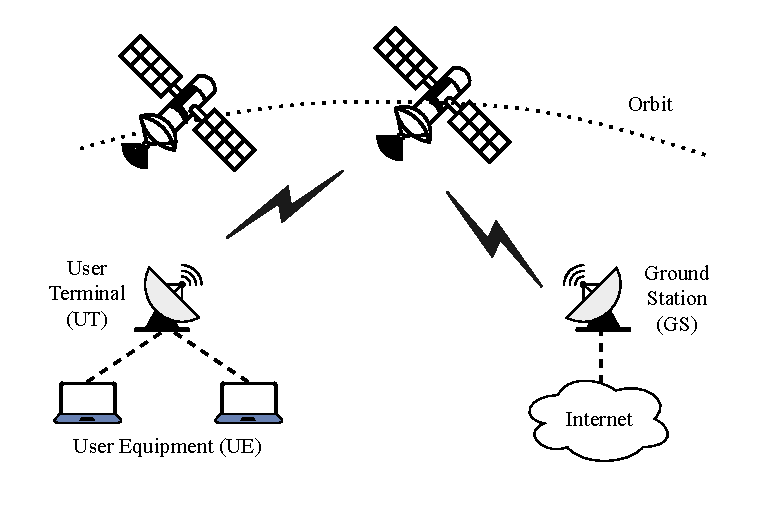
\includegraphics[width=0.5\linewidth]{figures/Satcom_modeling_diagram.pdf}
    \caption{Overview of the LEO SatCom network}
    \label{fig:Satcom_modeling_diagram}
\end{figure*}


\subsubsection{Temporal dynamics characteristics} 

LEO SatCom links exhibit \textbf{structured, time-varying dynamics} that come from satellite motion and gateway/Point-of-Presence (PoP) selection, on top of \textbf{stochastic effects} such as rain fade and interference. Unlike terrestrial links, LEO dynamics exhibit {periodic patterns} via predictable orbital paths, overlaid with stochastic impairments that correlate with physical-layer (PHY) changes in SINR and handover.  

Temporal dynamics manifest in critical network performance indicators including round-trip time (RTT), packet loss, and throughput. Their dynamic characteristics are listed as follows:

\begin{enumerate}
    \item \textbf{RTT}: LEO RTT exhibits continuous variations due to multiple factors of the LEO link, e.g., routing changes, rain fade, and short-term congestion \cite{chen2025minimum}. Sharp latency spikes are a consistent feature and are strongly correlated with handover events to the next rising satellite \cite{tian2025attention}.
    \item \textbf{Packet Loss}: LEO packet loss tends to be bursty rather than uniformly distributed, often occurring during handover or congestion transitions \cite{li2024satguard}.
    \item \textbf{Throughput}: LEO throughput shows multi-timescale fluctuations: (1) periodic short-term (seconds level) variability caused by network reconfiguration events, (2) longer-term shifts associated with load balancing/congestion during peak vs. non-peak hours, and (3) daily moderate attenuation due to weather effects like rainfall.
    \item \textbf{Time of Day}: Due to user's sharing satellites and limited routes and bandwidth compared to terrestrial, time of day has significant impact on throughput. For Starlink, we see 2:00 -- 5:00 a.m. having throughput highs of 200 -- 375 Mbps and lows of 30 -- 240 around 8:00 p.m. \cite{liu2025vivisecting}.
\end{enumerate}

To summarize, LEO temporal dynamics are not random but results from the superposition of scheduling periodicity, orbital motion, load balancing, and environmental factors, creating a highly volatile yet partially predictable temporal structure.

\subsubsection{OneWeb vs. Starlink Temporal Dynamics}

OneWeb and Starlink are two leading LEO satellite network service providers with 10375 and 654 active satellites\footnote{https://satellitemap.space/constellation/starlink}, respectively, as of May 2026. While both are LEO constellations, their temporal dynamics differ due to altitude and scheduler design. Their comparisons are:
\begin{itemize}
    \item \textbf{Shorter RTT of Starlink than OneWeb}: As shown in Table~\ref{tab:lsns}, Starlink operates at a lower altitude (~550 km), resulting in shorter propagation distance and further lower latency. Measurement studies show that Starlink has a median RTT of 25-60 ms \cite{Ullah2025inflight}, whereas Oneweb presents a longer 50-100 ms \cite{zhao2025measuring}.
    \item \textbf{15-second reconfiguration cycle of Starlink} \cite{garcia2023multi, tian2025attention}: Specific to Starlink is its 15-second reconfiguration schedule. Starlink addresses frequent beam and satellite transitions with the 15-second reconfiguration mechanism during which it recomputes the user-satellite assignment. Its scheduler requires a fixed 15-second cycle for reconfiguration to ensure service continuity, yet notable degradation in RTT and throughput. This phenomena occurs even if the serving satellite is the same, with the degredation in this case due to beam switching in the satellite rather than a handover to a different satellite.
    \item \textbf{Similar weather-induced channel variation}: Both Starlink and OneWeb use Ku/Ka bands, making them similarly susceptible to weather-induced temporal fading.
\end{itemize}

Figure~\ref{fig:Starlink_OneWeb} shows the collocated ready-to-use Starlink and OneWeb UTs on ARA. This setup enables controlled, side-by-side comparative analysis of the two LEO systems under identical environmental and traffic conditions. It further supports use cases, including (1) validation of temporal dynamics prediction models with improved generalization across both LEO constellations, and (2) traffic steering across the two satellite links


\begin{figure*}
    \centering
    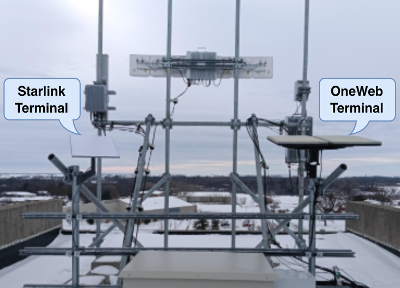
\includegraphics[width=0.5\linewidth]{figures/starlinkandonewebUT.png}
    \caption{Collocated UTs for Starlink (left) and OneWeb (right) available on the ARA Wireless Living Lab, enabling side-by-side comparative analysis.}
    \label{fig:Starlink_OneWeb}
\end{figure*}


\section{Modeling Review}

\subsection{5G Modeling}

For 5G and LTE, throughput is largely determined by observable radio-layer state (CQI, RSRP, RSRQ, SINR, MCS, etc) which maps well to tree-based models. The authors of \cite{minovski2021throughput} achieve $93\% \text{ R}^2$ with XGBoost using these features directly, and Lumos5G \cite{lumos5g} chooses GDBT for the same reasons: lightweight, composable, and interpretable. 5G (mmWave) breaks these assumptions, where geolocation by itself is insufficient and no single feature group dominates. This motivates the usage of Seq2Seq components for trajectory-based regression seen in \cite{lumos5g} and TPA-LSTM for mobility scenarios where temporal patterns recur \cite{MEI2022108736}. An observation from \cite{10723472} is that fine-grained cellular throughput may be inherently unpredictable because nearly identical historical sequences can produce wildly different next samples, limiting achievable accuracy regardless of model sophistication.

\subsection{Starlink Modeling}

Starlink's dominant variability source is network-level: the 15-second global rescheduling cycle, satellite load balancing, and weather attenuation. StarNet \cite{liu2025vivisecting} addresses this with a GRU-based Seq2Seq and custom periodical embedding, explicitly encoding the scheduling period rather than hoping the network learns it implicitly; ablations show that removing the embedding causes the model to attend to the wrong part of the window, degrading accuracy by over 13\%. T3P \cite{tiwari_t3p_2023} finds that XGBoost and LSTM are both viable for Starlink prediction using satellite trajectory features and past telemetry, with XGBoost outperforming LSTM on throughput and LSTM winning on latency. ASTM \cite{Tian2025attentionbased} extends the spatiotemporal approach further by combining a two-layer Transformer with Dynamic Graph Convolutional Networks to jointly model handover cycles and evolving satellite geometry, outperforming vanilla LSTM by 49\% on long-term RTT prediction.

\subsection{OneWeb Modeling}

OneWeb represents a distinct and largely unmodeled LEO satellite network. Its 16-beam per satellite design and near-polar orbits at 1,200 km produce periodic inter-beam handovers, but the more disruptive events are SNP (Satellite Network Portal) handovers (same as ground stations for Starlink), driven by ground infrastructure geography rather than satellite motion. These SNP handovers create two distinct latency distributions with no direct Starlink analog \cite{zhao2025measuring, 11310330}. The absence of ISLs means latency variation is partly a function of which coastal ground station is in line-of-sight, introducing geographic dependency that purely temporal models cannot capture. In \cite{11310330} we observed that although handovers are periodic, performance dips remain "not clearly predictable," which echos \cite{10723472} finding for 5G. We have not found dedicated predictive modeling work on OneWeb other than our current work.
    
\section{Bridging the Gap}    

The link dynamics across these three systems map directly onto model architectural choices in ways that reveal both what the literature has gotten right and where it falls short. In 5G, dynamics are dominated by stochastic radio variation (mobility, shadowing, and interference) which are well-captured by observable KPIs (SINR, CQI, MCS), explaining why tree-based models suffice under stable conditions \cite{minovski2021throughput, lumos5g}. When mmWave introduces blockage sensitivity and non-stationarity, temporal models become necessary \cite{lumos5g, MEI2022108736}, but \cite{10723472} shows that when the channel changes faster than the observation window, no architecture resolves the ambiguity. 

In Starlink, the 15-second reconfiguration cycle is deterministic and scheduler-imposed, which is why explicitly encoding it as a structural prior outperforms learning it from data \cite{liu2025vivisecting}; the residual error reflects slower, less structured load and weather components. ASTM's spatiotemporal approach \cite{Tian2025attentionbased} further addresses the geometric component of LEO dynamics (satellites moving at ~7--8 km/s), which purely temporal models systematically underfit. 

OneWeb occupies a third condition: its latency volatility is driven primarily by SNP selection, a geographic event determined by ground station line-of-sight rather than a repeating schedule \cite{zhao2025measuring, 11310330}. The dominant predictive feature may therefore be spatial geometry, not temporal history, although no model in the literature represents this. We do see peridic handovers of course with OneWeb, however its make-before-break behavior significatly minimizes its impact (especially compared to Starlink). We also see periodic SINR dips which remain to be investigated, they are currently believed to be due the satellite switching which beam it uses to communicate with the UT on the ground. We also note data scarcity from OneWeb's network in public research. Overall, the field has made the most progress where the primary dynamic is either well-instrumented (5G) or structurally encodable (Starlink), and the open areas are where it is spatial and data-scarce.

\section{Data Collection}

\subsection{Network Architecture Setup}

For our modeling data collection, we have one holistic data collection framework currently supporting Starlink and our mid-band 5G network. Our OneWeb access is currently unavailable so we do not include this in our current framework, however we will add it once we regain access. We do have some data from OneWeb to utilize from our year one work. Our network architectures are shown in Figs. \ref{fig:leo-arch} \& \ref{fig:5g-arch}, which showcases the setup used in our data collection. Fig. \ref{fig:5g-arch} showcases our 5G data collection setup which consists of our 5G user equipment (UE) (specifically a Quectel COTS UE) connecting to our 5G base station utilizing the mid-band frequency. From the base station the data traverses through the 5G core to our server. We therefore conduct our application experiments between the UE and our server. We deploy our data collection software for 5G at four different UE sites to add variety to our data set. It is important to note these UE sites are STATIC and not mobile, a dataset consisting of mobile UEs would be much more beneficial for developing models to be used in mobile scenarios.

\begin{figure}[htbp]
    \centering
    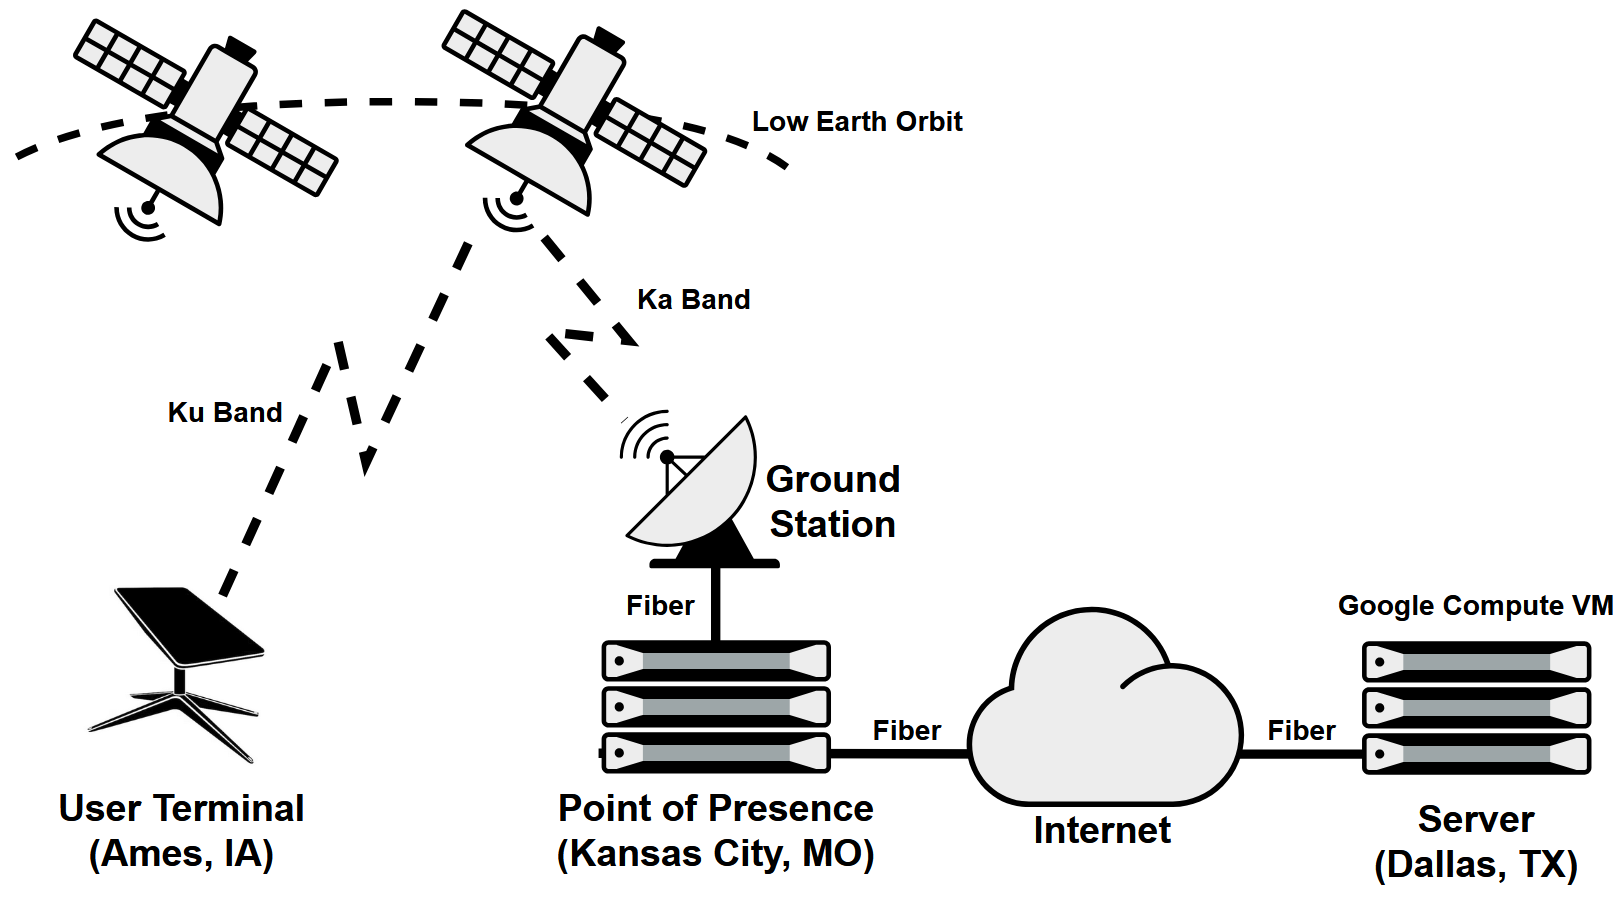
\includegraphics[width=0.75\linewidth]{figures/leo_arch.png}
    \caption{ARA's LEO network architecture for data collection 
    }
    \label{fig:leo-arch}
\end{figure}

We have a similar setup for our LEO satellite experiments as shown in Fig. \ref{fig:leo-arch}, conducting our experiments between our user terminal (UT) and our server. A little different, due to the nature of not having access to Starlink's private network, we host a public IP server using Google's compute resources. Our data flow here is therefore from our UT to the satellite, then to a ground station (GS) which then routes traffic to one of Starlink's points of presence (PoP), which then accesses the Internet to our server. While the internal Starlink network (UT - Satellite - GS - PoP) is out of our control, we do have some understanding of the internals. First, the GS is selected dynamically based on the satellites choice using its own positioning; therefore the GS choice is out of our control and unknown to us. Second, the PoP is fixed once the UT connects to Starlink's network for the first time. This will not change unless Starlink establishes new PoP's closer to our UT and reconfigures their network \cite{pan_measuring_2024}. Utilizing traceroute and other tools, we know our associated PoP is in Kansas City, MO. Unfortunately, there is no Kansas City, MO data center provided by any of the big compute server providers (Google, AWS, Azure, etc), therefore we have selected to reserve a Google compute server located in Dallas, TX as our server for our data collection experiments. Another option is Council Bluffs, IA, however we did not notice any prominent latency differences between Dallas and Council Bluffs.

As of May 2026, Starlink and OneWeb differ in the capacities showcased in Table \ref{tab:lsns}.

\begin{figure}[htbp]
    \centering
    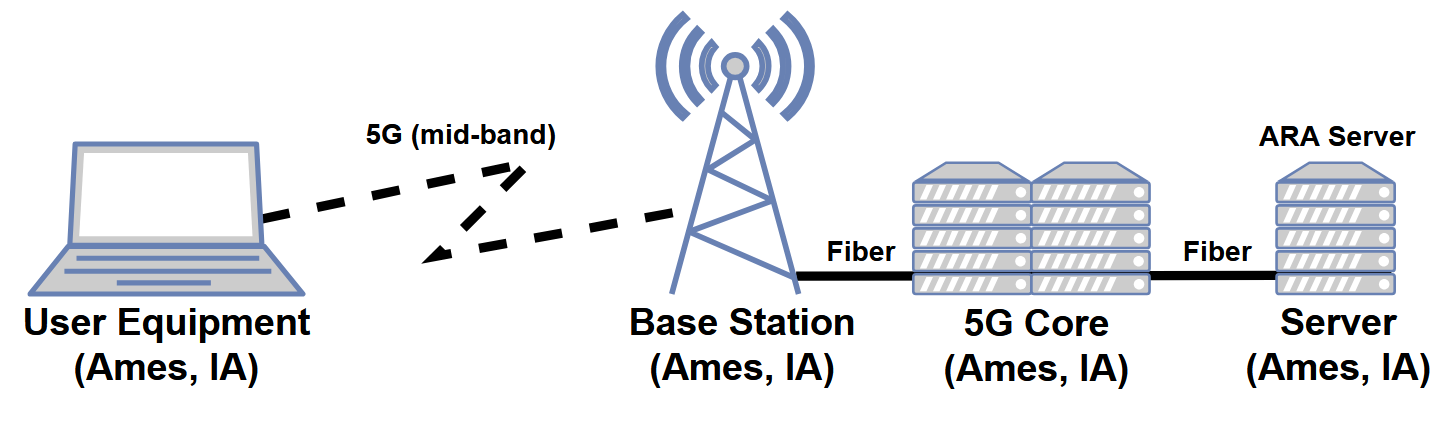
\includegraphics[width=0.75\linewidth]{figures/5g_arch.png}
    \caption{ARA's 5G network architecture for data collection 
    }
    \label{fig:5g-arch}
\end{figure}

% \begin{figure}[htbp]
%     \centering
%     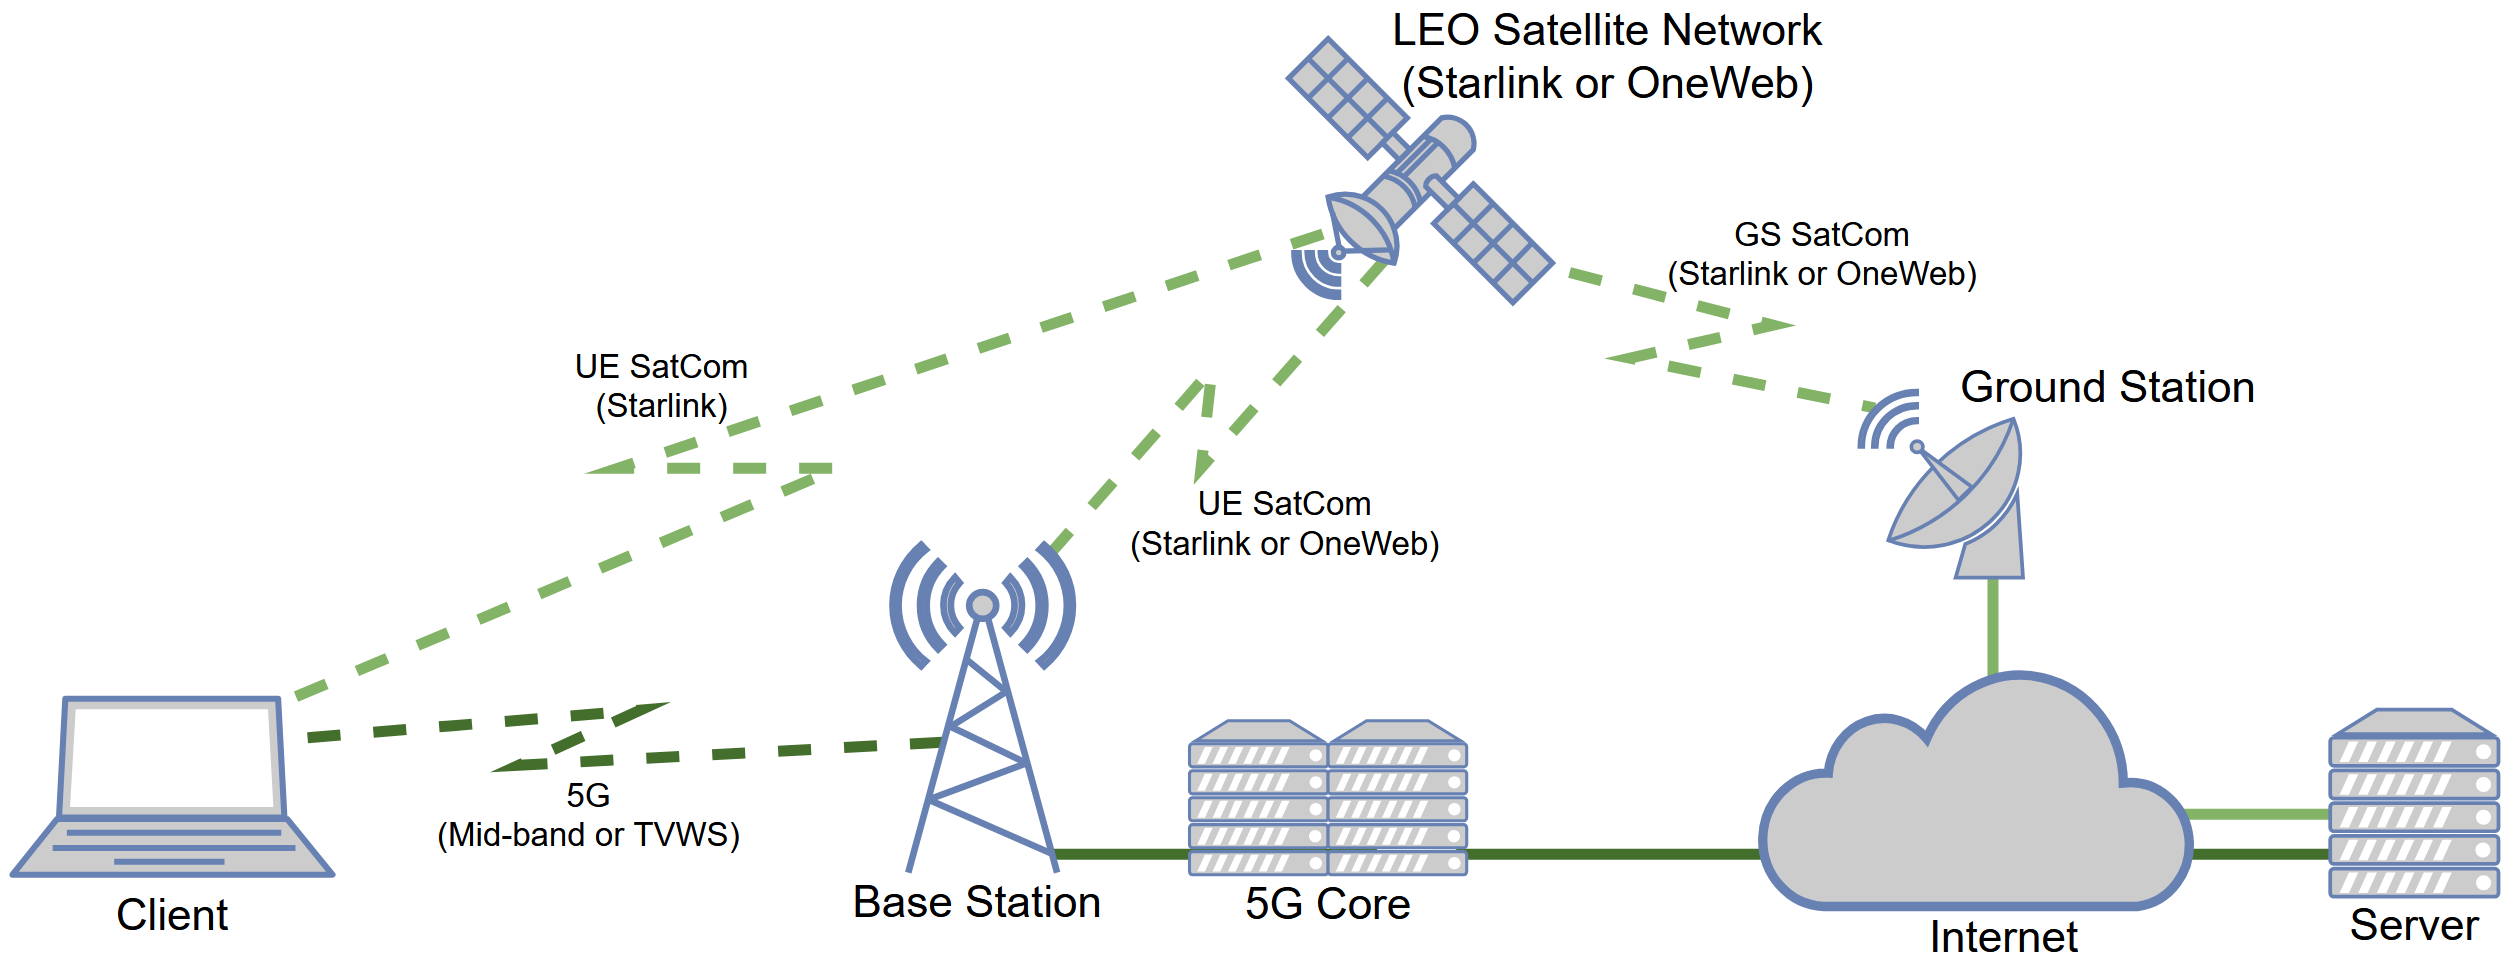
\includegraphics[width=0.75\linewidth]{figures/stin-arch.png}
%     \caption{ARA's Space-Terrestrial Integrated Network 
%     }
%     \label{fig:stin-arch}
% \end{figure}

\begin{table}[htpb]
    \centering
    \resizebox{\columnwidth}{!}{
    \begin{tabular}{|c|c|c|c|c|c|c|}
         \hline
         \textbf{LSN} & \textbf{UE Spectrum} & \textbf{GW Spectrum} & \textbf{\# of Satellites} & \textbf{Altitude (km)} & \textbf{Latency (ms)}  \\
         \hline
         Starlink & Ku Band & Ka Band & 10375 & $\approx550$ & 20-40 \\
         \hline
         OneWeb & Ku Band & Ka Band & 654 & $\approx1200$ & 50 \\
         \hline
    \end{tabular}
    }
    \caption{Starlink and OneWeb LEO Satellite Network (LSN) comparison}
    \label{tab:lsns}
\end{table}

\subsection{Application Software Setup}

The data collection framework consists of two parallel pipelines, one for 5G over mid-band and one for our Starlink UT, both orchestrated by a common scheduling and execution layer.

Each pipeline is structured in three tiers. The top tier is a schedule controller that fires experiment slots at fixed times of day using a polling scheduler. At each slot, a main controller sequences the experiment, conducting a latency test, followed by a latency and loss test (using low throughput values to ensure available bandwidth for the latency), and finishing with a throughput test to capture max bandwidth availability. We utilize Linux's ping and iPerf3 tools to capture our latency and throughput respectively. With all experiments, we collect current weather data along side physical layer radio metrics (for 5G) and user terimal/satellite metrics (for Starlink). Each test block runs all collectors simultaneously (ex. weather, radio, latency) for ten minutes.

The bottom tier consists of the individual collectors, each implemented as a standalone Python subprocess. The iperf3 collector drives bidirectional throughput tests and captures per-interval throughput, jitter, packet loss, and RTT from both client and server sides. We run iPerf3 using only UDP currently to collect total bandwidth and accurate link packet losses. The ping collector issues ICMP probes at 200ms intervals to various servers. For 5G, it only collects latency to our sever; for Starlink we run three ping collectors: 1) to our server through our Wireguard tunnel (used to conduct throughput tests to the public IP server), 2) to our server through Starlink (no tunnel), and 3) to Cloudflare's DNS server located in Kansas City, MO to measure PoP only latency. 

The weather collector polls the ARA wireless living lab weather station at one-second intervals. For 5G, the radio collector retrieves per-sample RSRP, RSRQ, SINR, cell ID, ARFCN, and band metrics; the Starlink collector polls the dish's gRPC API at 200ms intervals for obstruction statistics, alignment, and GPS state. We run another collector as a satellite tracker which uses our UT's obstruction map and conducts frame analysis using TLE-based orbit propagation to identify the connected satellite and compute its position and distance at each timeslot.

All collectors write synchronized UTC timestamps and a shared experiment timestamp to enable cross-collector alignment during analysis.

\subsection{Collected Metrics}

The metrics we collect are listed in Table \ref{tab:metrics}. The 5G and LEO satellite metrics are of course subject to the provider and hardware, so a different 5G radio may expose more or less physical layer information, same with LEO satellite network providers. They are also subject to change, for example Starlink used to provide SINR in its API but has since removed that capability and we can now only see a boolean value dictating whether or not it is above the noise floor. Furthermore teh satellite tracker information for Starlink utilized Starlink TLE information and algorithms from \cite{pan_measuring_2024} to estimate which Starlink satellite the UT is currently connected to. 

\begin{table*}[t]
\centering
\caption{Collected Metrics by Platform and Collector}
\label{tab:metrics}
\renewcommand{\arraystretch}{1.2}
\setlength{\tabcolsep}{5pt}

\begin{tabular}{p{2.2cm} p{2.5cm} p{10.8cm}}
\toprule
\textbf{Platform} & \textbf{Collector} & \textbf{Collected Metrics} \\
\midrule

\multirow{3}{*}{Common}
& \texttt{iperf3}
& Throughput, jitter, packet loss \\

& \texttt{ping}
& Latency (RTT) \\

& \texttt{weather}
& Temperature, humidity, pressure, wind speed/direction, rain rate, rain accumulation \\

\midrule

\multirow{1}{*}{5G}
& \texttt{radio}
& RSRP, SINR, Cell ID, ARFCN, band \\

\midrule

\multirow{2}{*}{Starlink}
& \texttt{terminal}
& Terminal obstruction fraction, obstruction duration, SNR above noise floor, desired/actual azimuth \& elevation, tilt angle \\

& \texttt{satellite tracker}
& Satellite ID, distance, elevation angle, azimuth angle, satellite latitude/longitude/altitude \\

\midrule

\multirow{2}{*}{OneWeb}
& \texttt{terminal}
& RSRP, RSRQ, SINR, RSSI, desired/actual azimuth \& elevation, satellite ID, track ID, beam switch time, distance, elevation angle, Rx/Tx tuning frequency \\

\bottomrule
\end{tabular}

\end{table*}

\section{Modeling}

\subsection{Our Models}
The framework evaluates five model families spanning classical statistical approaches, shallow machine learning, and deep sequence models. Together they form a structured comparison: strong sequential models serve as primary candidates for high-performance predictions, while simpler models establish our baselines. We also adapt some models from \cite{liu2025vivisecting} and include their results (labeled as Starnet-model). These are adapted to our framework, datasets, and modeling methodologies and therefore not completely indicative of their original performance, which is quite high as shown in their paper.

\begin{itemize}

\item \textbf{Seq2Seq-GRU} — The primary model and main experimental candidate. A two-layer GRU encoder processes the input window concatenated with a learned periodic time embedding: a small \texttt{Linear(4, embed\_dim)} layer projects four sin/cos encodings of hour-of-day and
day-of-week into a compact representation. A two-layer GRU decoder with additive (Bahdanau) attention auto-regressively produces all horizon steps, with one projection head per target for simultaneous multi-target forecasting (MIMO). Teacher forcing is annealed over training, and the training loop additionally applies exponential moving average smoothing. This model is expected to perform best and is the subject of the feature and architecture ablation studies.

\item \textbf{LSTM} — A competitive deep-learning baseline. A two-layer LSTM with dropout appends four raw sin/cos cyclical encodings of hour-of-day and day-of-week directly to the feature tensor. The final hidden state is projected by a single \texttt{Linear} head to \texttt{output\_len
$\times$ num\_targets} values and reshaped, producing all horizon steps and targets jointly in one forward pass (MIMO). It shares the same training loop and hyperparameter configuration as the Seq2Seq model, isolating the contribution of the encoder-decoder structure and attention mechanism.

\item \textbf{Transformer} — A second competitive deep-learning baseline. An encoder-only Transformer appends the same four raw sin/cos time encodings as the LSTM, then projects the fused input to \texttt{d\_model} dimensions and adds a \emph{learned} positional encoding (a \texttt{register\_buffer} initialized with $\mathcal{N}(0, 0.02)$, kept small to avoid dominating
early training). Multi-head self-attention over the full input sequence reads the final token's representation, which a single MIMO linear head projects to all horizon steps and targets simultaneously. Training includes a wall-clock timeout to prevent runaway runtimes on large configurations.

\item \textbf{Gaussian Process} — A probabilistic shallow baseline. The input windows (flattened to \texttt{seq\_len $\times$ num\_features}) are first standardized with \texttt{StandardScaler} and then reduced with PCA (default 50 components) before fitting, which manages the $O(n^3)$ cost and gives the RBF kernel meaningful geometry. One \texttt{GaussianProcessRegressor} with a \texttt{ConstantKernel $\times$ RBF} kernel, \texttt{normalize\_y=True}, and two optimizer restarts is then fit independently per horizon step (MISO) on a subsampled snapshot of the training set. Its primary role is to quantify uncertainty and provide a well-calibrated probabilistic lower bound on achievable performance, rather than to compete on raw accuracy at scale.

\item \textbf{Predictive Autoencoder} — An unsupervised-pretraining baseline, available in three variants. All share the same two-layer encoder/decoder/predictor structure: the full flattened input window (\texttt{seq\_len $\times$ num\_features}) is passed through two linear layers with ReLU activations to a bottleneck latent code, which is then decoded back to the input and separately mapped to the prediction. Training minimizes a weighted sum of MSE prediction loss and MSE reconstruction loss (\texttt{recon\_weight} controls the balance). The three variants differ only in how the latent code is regularized: \emph{standard} applies no additional penalty; \emph{sparse} adds an L1 penalty on the mean absolute activation of the latent vector; \emph{variational} uses the reparameterization trick with a $\beta$-weighted KL divergence term (a $\beta$-VAE). Included to assess whether learning a compressed latent representation of the input window is beneficial compared to direct sequence modeling.

\end{itemize}

\subsection{Features}
\label{subsec: features}

While not all will be utilized, we list the candidate features to train the models below. The default input features for Starlink, OneWeb, and 5G model training are indicated by \textbf{[S, O, Q]} respectively. 

\begin{itemize}
    \item \textbf{Network Performance}
    \begin{itemize}
        \item \textbf{[S, Q, O]} iPerf-measured throughput (Mbps)
        \item \textbf{[S, Q, O]} iPerf-measured jitter (ms)
        \item \textbf{[S, Q, O]} iPerf-measured packet loss (\%)
        \item \textbf{[S]} UT measured PoP latency (ms)
        \item \textbf{[S]} RTT to DNS server near PoP (ms)
        \item \textbf{[S, Q, O]} RTT to server endpoint (ms)
        
    \end{itemize}
    \item \textbf{Weather}
    \begin{itemize}
        \item Ambient temperature (\textdegree F)
        \item \textbf{[S, Q]} Relative humidity (\%)
        \item \textbf{[S, Q]} Atmospheric pressure (hPa)
        \item Wind speed (mph)
        \item Wind direction (degrees)
        \item \textbf{[S, Q]} Precipitation rate (mm/hr)
    \end{itemize}
    \item \textbf{Satellite Geometry}
    \begin{itemize}
        \item \textbf{[S]} Slant range from dish to satellite (km)
        \item Satellite latitude (degrees)
        \item Satellite longitude (degrees)
        \item Satellite altitude (km)
        \item \textbf{[S]} Satellite distance (km)
        \item \textbf{[S, O]} Elevation angle (degrees)
        \item \textbf{[S, O]} Azimuth angle (degrees)
    \end{itemize}
    \item \textbf{Signal Quality}
    \begin{itemize}
        \item \textbf{[S]} Signal-to-noise ratio at the dish (dB)
        \item \textbf{[O]} Signal-to-interference-plus-noise ratio (dB)
        \item \textbf{[Q]} Reference signal received power (dBm)
        \item \textbf{[Q]} Reference signal received quality (dB)
        \item \textbf{[Q]} Signal-to-interference-plus-noise ratio (dB)
    \end{itemize}
    \item \textbf{Dish State}
    \begin{itemize}
        \item Number of GPS satellites in view
        \item \textbf{[S]} Dish boresight azimuth (degrees)
        \item \textbf{[S]} Dish boresight elevation angle (degrees)
        \item Physical tilt angle of the dish (degrees)
        \item \textbf{[S]} Fraction of sky view obstructed (0--1)
    \end{itemize}
    \item \textbf{Satellite Metadata}
    \begin{itemize}
        \item \textbf{[S, O]} Binary indicator of a satellite handover
        \item \textbf{[S, O]} Time elapsed since last handover (s)
    \end{itemize}
\end{itemize}

\subsection{Training Framework}

\subsubsection{Overview}

The training pipeline is implemented as a unified framework supporting three prediction modes that govern the shape of model inputs and outputs throughout training and evaluation. These modes are Multi-Input Multi-Output (MIMO), Multi-Input Single-Output (MISO), and Single-Input Single-Output (SISO). Each mode imposes a strict tensor shape contract between the dataset, the model's output head, and the loss computation, ensuring architectural consistency across all experiments.

For MIMO and MISO, the models take the same feature inputs as specified in Section \ref{subsec: features}, but with multi- and single-output differences. For MIMO, \textbf{the target outputs are RTT, jitter, and packet loss}; and for MISO, the target is RTT. The throughput modeling can use some refinement, and as far as multipath packet scheduling, these are the key metrics to keep in mind. We did not implement a SISO model for this current analysis. 

\subsubsection{Prediction Modes}
\begin{itemize}
\item \textbf{MIMO (Multi-Input Multi-Output)} — In MIMO mode, the model consumes a multivariate input sequence of length $L_{\text{in}}$ and produces a full forecast tensor of shape $(B,\, H,\, T)$, where $B$ is the batch size, $H = L_{\text{out}}$ is the forecast horizon, and $T$ is the number of prediction targets. This mode is used by sequence-to-sequence, LSTM, Transformer, attention-based, and StarNet architectures. It is the default mode for multi-step, multi-target forecasting.

\item \textbf{MISO (Multi-Input Single-Output)} — MISO models consume multivariate input but produce a one-step-ahead prediction of shape $(B,\, T)$. Multiple targets are supported, with each target receiving its own output scalar per sample. This mode is used by Gaussian process, autoencoder, and MLP baseline models.

% \item \textbf{SISO (Single-Input Single-Output)} — SISO is the most constrained mode, accepting a single input feature and predicting a single scalar target per window. The input tensor is required to have exactly one feature channel, and the output matches the MISO shape $(B,\, L_{\text{out}})$. This mode is used by ARIMA-style statistical models. If a SISO model is requested with multiple targets, the framework automatically drops to the first target only.

\end{itemize}

\subsubsection{Loss Functions}

A mean squared error (MSE) criterion is used uniformly across all modes:
\[
    \mathcal{L} = \frac{1}{N}\sum_{i=1}^{N}\left(\hat{y}_i - y_i\right)^2.
\]
Mode-specific wrappers enforce the expected tensor shapes before computing the loss. In MISO 
% and SISO
mode, a trailing size-one dimension is automatically squeezed from the model output if present, converting an accidental $(B,\, H,\, 1)$ tensor to the required $(B,\, H)$ form. In MIMO mode, a strict shape equality check is applied and a descriptive error is raised on mismatch.

\subsubsection{Optimization}

All trainable models are optimized with AdamW using an initial learning rate $\eta = 10^{-3}$ and weight decay $\lambda = 10^{-3}$. Gradient norms are clipped to a maximum of $5.0$ to stabilize training. A \texttt{ReduceLROnPlateau} scheduler monitors the smoothed validation loss and reduces the learning rate by a factor of $0.5$ after $8$ epochs without improvement, down to a minimum of $10^{-6}$.

\subsubsection{Teacher Forcing}

For autoregressive MIMO models (e.g.\ the Seq2Seq-GRU), a teacher-forcing schedule is applied during training. The teacher-forcing ratio $\tau$ is annealed linearly from $0.5$ to $0$ over the first half of training:
\[
    \tau_e = \max\!\left(0,\; 0.5 \times \left(1 - \frac{e}{\lfloor E/2 \rfloor}\right)\right),
\]
where $e$ is the current epoch and $E$ is the total number of epochs. Teacher forcing is disabled entirely for MISO and SISO models.

\subsubsection{Early Stopping and Model Selection}

Validation loss is tracked using an exponential moving average (EMA) with smoothing factor $\alpha = 0.3$:
\[
    \tilde{\ell}_e = \alpha\,\ell_e + (1 - \alpha)\,\tilde{\ell}_{e-1},
\]
where $\ell_e$ is the raw validation loss at epoch $e$. The model checkpoint achieving the lowest smoothed validation loss $\tilde{\ell}$ is retained. Training is terminated early if no improvement is observed for $40$ consecutive epochs. At the end of training, the best checkpoint is reloaded before test-set evaluation.

\subsubsection{Data Splits and Normalization}

Each dataset is partitioned chronologically into training ($70\%$), validation ($15\%$), and test ($15\%$) splits. Input features and prediction targets are normalized prior to training using either $z$-score standardization,
\[
    \tilde{x} = \frac{x - \mu}{\sigma},
\]
or min-max scaling,
\[
    \tilde{x} = \frac{x - x_{\min}}{x_{\max} - x_{\min}},
\]
with statistics computed exclusively on the training partition. Predictions are de-normalized back to the original scale before metric computation.

\subsection{Evaluation}

After training, the best checkpoint is used to collect predictions over the held-out test set. Raw prediction and target tensors are converted to per-horizon dictionaries keyed by strings of the form \texttt{t+$k$s} (e.g.\ \texttt{t+1s}, \texttt{t+2s}, \ldots) for single-target experiments, or \texttt{<target>\_t+$k$s} for multi-target experiments. Metrics including MAE, RMSE, $R^2$, and the $95\%$ prediction interval coverage probability (PICP$_{95}$) are then computed per horizon and aggregated across the full forecast window.

\section{Results}

\subsection{Modeling Performance}

Tables~\ref{tab:results_oneweb}, \ref{tab:results_5g}, and~\ref{tab:results_starlink} summarize the predictive performance of all evaluated models across three satellite constellations (OneWeb, 5G, Starlink) and both link directions (downlink and uplink), measured by MAE, RMSE, MAPE, sMAPE, R\textsuperscript{2}, PICP\textsubscript{95}, and MIS.

\paragraph{Overall Rankings.}
Across all six dataset configurations, the sequence-to-sequence family of models (Seq2Seq-GRU, StarNet-GRU, StarNet-ATTENTION) consistently achieve the lowest point-error metrics and highest R\textsuperscript{2} scores among all evaluated architectures. Seq2Seq-GRU ranks first or within a narrow margin of first on MAE and RMSE in five of the six configurations, with StarNet-GRU occasionally edging it out by a small margin. StarNet-ATTENTION performs comparably to StarNet-GRU on interval quality (MIS), producing the lowest MIS on OneWeb UL (325.8) and 5G UL (39.3). The standard LSTM and Transformer models trail the GRU-based approaches across the board, particularly on uplink tasks, suggesting that recurrent inductive biases tailored to sequential satellite telemetry are beneficial.

% ── TABLE 1: OneWeb ──────────────────────────────────────────────────────────
\begin{table}[ht]
\centering
\caption{%
  Model performance on the \textbf{OneWeb} constellation (DL and UL).
  \best{Bold}: best per column; \second{underline}: second best.
  Negative R\textsuperscript{2} indicates worse than the naive mean predictor.
}
\label{tab:results_oneweb}
\setlength{\tabcolsep}{4pt}
\renewcommand{\arraystretch}{1.15}
\small
\begin{tabular}{ll rrrrr r}
\toprule
\textbf{Dir.} & \textbf{Model}
  & \textbf{MAE} & \textbf{RMSE} & \textbf{MAPE} & \textbf{sMAPE}
  & \textbf{R\textsuperscript{2}} & \textbf{MIS} \\
  & & & \textbf{(\%)} & \textbf{(\%)} & & \textbf{95} & \\
\midrule

\multirow{8}{*}{\rotatebox[origin=c]{90}{\textbf{DL}}}
  & Seq2Seq-GRU         & \second{6.12}  & \second{23.73} & \second{43.61} & \second{85.25} & \second{0.217} & \second{108.69} \\
  & LSTM                & 6.69           & 25.63          & 47.66          & 87.08          & 0.110          & 129.55          \\
  & Transformer         & 6.21           & 25.17          & 44.59          & 85.47          & 0.188          & 114.08          \\
  & StarNet-GRU       & \best{5.96}    & \best{23.59}   & \best{43.13}   & 85.63          & \best{0.223}   & \best{103.93}   \\
  & StarNet-ATTENTION & 6.87           & 23.75          & 45.57          & 86.60          & 0.221          & 109.45          \\
  & StarNet-FNN       & 8.70           & 26.46          & 49.89          & 90.03          & 0.147          & 114.88          \\
  & GaussianProcess     & 24.26          & 76.86          & 30.30          & \best{28.18}   & $-$0.003       & 324.46          \\
  & Autoencoder         & 18.06          & 69.23          & \best{20.06}   & \second{18.91} & 0.165          & 334.31          \\
\midrule

\multirow{8}{*}{\rotatebox[origin=c]{90}{\textbf{UL}}}
  & Seq2Seq-GRU         & \second{22.81} & \second{49.40} & \second{28.15} & \best{8.42}    & \second{0.918} & \second{337.12} \\
  & LSTM                & 33.42          & 68.66          & 46.68          & 10.95          & 0.851          & 487.78          \\
  & Transformer         & 32.87          & 67.84          & 48.42          & 10.71          & 0.855          & 484.34          \\
  & StarNet-GRU       & 23.41          & \best{48.89}   & 31.27          & 9.58           & \best{0.920}   & 334.48          \\
  & StarNet-ATTENTION & 24.35          & 49.02          & 34.58          & 9.66           & 0.919          & \best{325.80}   \\
  & StarNet-FNN       & 32.40          & 56.78          & 49.29          & 12.73          & 0.893          & 364.48          \\
  & GaussianProcess     & 171.13         & 284.66         & 76.82          & 63.03          & 0.136          & 1612.85         \\
  & Autoencoder         & 88.83          & 181.16         & \second{39.43} & \second{30.37} & 0.628          & 1268.21         \\

\bottomrule
\end{tabular}

\smallskip
\noindent\footnotesize
Note: PICP\textsubscript{95} $\approx 0.950$ uniformly across all models and datasets,
confirming well-calibrated intervals. MAPE and sMAPE are inflated by near-zero throughput
values in some datasets (see text); MAE, RMSE, and R\textsuperscript{2} are the primary
discriminating metrics.
\end{table}


% ── TABLE 2: 5G ─────────────────────────────────────────────────────────
\begin{table}[ht]
\centering
\caption{%
  Model performance on the \textbf{5G} constellation (DL and UL).
  \best{Bold}: best per column; \second{underline}: second best.
  Negative R\textsuperscript{2} indicates worse than the naive mean predictor.
}
\label{tab:results_5g}
\setlength{\tabcolsep}{4pt}
\renewcommand{\arraystretch}{1.15}
\small
\begin{tabular}{ll rrrrr r}
\toprule
\textbf{Dir.} & \textbf{Model}
  & \textbf{MAE} & \textbf{RMSE} & \textbf{MAPE} & \textbf{sMAPE}
  & \textbf{R\textsuperscript{2}} & \textbf{MIS} \\
  & & & \textbf{(\%)} & \textbf{(\%)} & & \textbf{95} & \\
\midrule

\multirow{8}{*}{\rotatebox[origin=c]{90}{\textbf{DL}}}
  & Seq2Seq-GRU         & \second{1.10}  & \second{1.66}  & \second{55.31} & \second{78.49} & \second{0.273} & \second{8.94}  \\
  & LSTM                & 1.12           & 1.70           & 59.76          & 79.32          & 0.129          & 9.25           \\
  & Transformer         & 1.18           & 1.71           & 59.31          & 79.78          & 0.227          & 8.89           \\
  & StarNet-GRU       & 1.11           & \best{1.66}    & 56.23          & 78.54          & 0.270          & 8.93           \\
  & StarNet-ATTENTION & \best{1.10}    & \best{1.66}    & \best{55.85}   & 78.90          & \best{0.274}   & \best{8.88}    \\
  & StarNet-FNN       & 1.34           & 1.90           & 67.54          & 81.02          & 0.087          & 9.15           \\
  & GaussianProcess     & 3.67           & 5.11           & \second{28.42} & \second{25.99} & 0.068          & 25.32          \\
  & Autoencoder         & 3.23           & 4.63           & \best{25.39}   & \best{22.89}   & 0.233          & 24.68          \\
\midrule

\multirow{8}{*}{\rotatebox[origin=c]{90}{\textbf{UL}}}
  & Seq2Seq-GRU         & \second{4.40}  & \second{7.91}  & \second{61.45} & \second{90.55} & \second{0.114} & \second{39.35} \\
  & LSTM                & 4.46           & 8.09           & 63.21          & 91.17          & 0.015          & 42.09          \\
  & Transformer         & 4.45           & 7.95           & 62.57          & 91.61          & 0.101          & 39.52          \\
  & StarNet-GRU       & 4.44           & 7.91           & 62.12          & 91.56          & 0.115          & 39.50          \\
  & StarNet-ATTENTION & \best{4.36}    & \best{7.90}    & \best{61.36}   & \best{91.15}   & \best{0.118}   & \best{39.27}   \\
  & StarNet-FNN       & 4.60           & 8.88           & 67.30          & 92.59          & $-$1.067       & 41.18          \\
  & GaussianProcess     & 12.34          & 20.10          & \second{85.29} & \second{62.29} & $-$0.004       & 96.48          \\
  & Autoencoder         & 12.77          & 53.65          & 91.43          & 61.70          & $-$6.189       & 114.87         \\

\bottomrule
\end{tabular}
\end{table}


% ── TABLE 3: Starlink ────────────────────────────────────────────────────────
\begin{table}[ht]
\centering
\caption{%
  Model performance on the \textbf{Starlink} constellation (DL and UL).
  \best{Bold}: best per column; \second{underline}: second best.
  Negative R\textsuperscript{2} indicates worse than the naive mean predictor.
}
\label{tab:results_starlink}
\setlength{\tabcolsep}{4pt}
\renewcommand{\arraystretch}{1.15}
\small
\begin{tabular}{ll rrrrr r}
\toprule
\textbf{Dir.} & \textbf{Model}
  & \textbf{MAE} & \textbf{RMSE} & \textbf{MAPE} & \textbf{sMAPE}
  & \textbf{R\textsuperscript{2}} & \textbf{MIS} \\
  & & & \textbf{(\%)} & \textbf{(\%)} & & \textbf{95} & \\
\midrule

\multirow{8}{*}{\rotatebox[origin=c]{90}{\textbf{DL}}}
  & Seq2Seq-GRU         & \second{8.55}  & \second{14.95} & \second{60.77} & \best{76.33}   & \second{0.406} & \second{98.37}  \\
  & LSTM                & 8.90           & 16.75          & 81.87          & 85.08          & $-$0.056       & 112.54          \\
  & Transformer         & 9.89           & 16.48          & 67.92          & 82.64          & 0.249          & 98.37           \\
  & StarNet-GRU       & 9.40           & 15.58          & \best{60.17}   & 85.15          & 0.390          & \best{94.98}    \\
  & StarNet-ATTENTION & \best{8.44}    & \best{14.91}   & 63.90          & 77.07          & 0.373          & 96.03           \\
  & StarNet-FNN       & 10.40          & 16.49          & 74.05          & 92.91          & 0.249          & 102.14          \\
  & GaussianProcess     & 38.25          & 50.34          & \second{57.11} & \second{41.75} & 0.348          & 243.29          \\
  & Autoencoder         & 19.65          & 36.21          & \best{26.99}   & \best{19.61}   & \best{0.660}   & 245.41          \\
\midrule

\multirow{8}{*}{\rotatebox[origin=c]{90}{\textbf{UL}}}
  & Seq2Seq-GRU         & \best{1.48}    & \best{3.18}    & \second{34.94} & \second{66.37} & \second{0.199} & \second{15.26}  \\
  & LSTM                & 1.54           & 3.36           & 36.03          & 66.12          & 0.092          & 17.03           \\
  & Transformer         & 1.50           & 3.27           & 36.31          & 68.97          & 0.166          & 15.79           \\
  & StarNet-GRU       & \second{1.48}  & \second{3.24}  & 42.32          & \best{65.35}   & 0.153          & 15.93           \\
  & StarNet-ATTENTION & 1.50           & 3.30           & 41.19          & 66.54          & 0.081          & 16.46           \\
  & StarNet-FNN       & 1.51           & 3.27           & \best{34.39}   & 65.76          & 0.122          & \best{15.55}    \\
  & GaussianProcess     & 5.19           & 8.28           & \second{13.19} & \second{13.08} & 0.110          & 42.32           \\
  & Autoencoder         & 3.96           & 7.19           & \best{9.79}    & \best{9.80}    & \best{0.329}   & 38.64           \\

\bottomrule
\end{tabular}

\end{table}

\paragraph{Baseline Comparison.}
The GaussianProcess and Autoencoder-standard baselines perform substantially worse on point-error metrics (MAE, RMSE) in all configurations. However, their MAPE and sMAPE figures are notably \emph{lower} on several datasets, particularly Starlink UL, where the Autoencoder achieves 9.8\% sMAPE compared to 65-69\% for the deep learning models. This apparent contradiction reflects the well-known sensitivity of percentage-based metrics to near-zero target values: when throughput measurements approach zero, deep learning predictions incur artificially inflated relative errors even if absolute deviations are small. The R\textsuperscript{2} and RMSE metrics, which are not distorted by this effect, confirm the superiority of the sequence models. 
% Notably, the Autoencoder achieves competitive R\textsuperscript{2} on Starlink DL (0.66), the highest of any model on that dataset, suggesting that its reconstruction-based objective may capture slow throughput dynamics in Starlink's highly variable downlink.

\paragraph{Dataset-Level Observations.}
The difficulty of the prediction task varies considerably by constellation and link direction. OneWeb UL exhibits the highest absolute RTT magnitudes and R\textsuperscript{2} values (up to 0.92), indicating a relatively structured and learnable signal. In contrast, OneWeb DL and 5G UL yield low R\textsuperscript{2} scores across all deep learning models (best: 0.27 and 0.12, respectively), pointing to high signal variability or limited autocorrelation at the chosen prediction horizon. Starlink DL presents a mixed picture: Seq2Seq-GRU achieves R\textsuperscript{2} = 0.41 while the Autoencoder reaches 0.66, suggesting that different aspects of the Starlink downlink distribution are captured by different model classes. Across all datasets, 5G RTT values operate at a much smaller absolute scale (MAE on the order of 1-4 ms for DL, 4-13 for UL), yet percentage errors remain high, reinforcing the zero-proximity artifact described above.

\paragraph{Calibration and Interval Quality.}
All models achieve near-nominal empirical coverage of 95.0\% (PICP\textsubscript{95} $\approx$ 0.950 across all entries), indicating that the prediction intervals are well-calibrated regardless of the model family. The discriminating metric is therefore MIS, which penalizes unnecessarily wide intervals. Seq2Seq-GRU and StarNet-GRU consistently produce the tightest intervals among the deep learning models. The GaussianProcess baseline generates the widest intervals by a large margin on five of six datasets (e.g., MIS = 1612.8 on OneWeb UL vs.\ 325.7-487.8 for deep learning models), reflecting its difficulty in scaling to high-dimensional, nonstationary satellite throughput distributions.

\paragraph{Summary.}
Taking point accuracy, explained variance, and interval sharpness together, Seq2Seq-GRU and StarNet-GRU emerge as the most reliable architectures across constellations and link directions. StarNet-FNN consistently underperforms relative to its recurrent counterparts despite sharing the same satellite-aware input features, suggesting that temporal sequence modeling is more important than feature engineering alone for this task. Given its performance consistency and architectural simplicity, Seq2Seq-GRU is selected for deeper analysis in the following subsection.

\subsection{Seq2Seq-GRU Performance Analysis}

The Seq2Seq-GRU model was selected for deeper analysis based on its consistent ranking among the top-performing architectures across constellations and link directions. The model operates in a MIMO (Multiple-Input Multiple-Output) configuration, simultaneously predicting three target variables—RTT, jitter, and packet loss—over a 15-second horizon using a single forward pass. The architecture contains approximately 449{,}000-457{,}000 trainable parameters depending on the feature set, which varies by provider. All models converged within 42-53 epochs, suggesting stable training dynamics and no apparent overfitting beyond early stopping. The scatter plots showing predicted vs. actual values are shown in Figs. \ref{fig:s2s_oneweb} - \ref{fig:s2s_starlink}.

\paragraph{Interpreting the Metrics.}
Before discussing results, it is useful to establish what constitutes strong performance for each metric in this context. An R\textsuperscript{2} value of 1.0 represents perfect prediction; values above 0.80 are generally considered strong for nonlinear time-series forecasting, 0.50--0.80 moderate, and below 0.50 weak, with negative values indicating the model performs worse than simply predicting the mean at every step. Relative RMSE (RMSE normalized by a naive baseline) below 1.0 confirms the model improves on persistence; values below 0.80 indicate meaningful improvement. Residual autocorrelation (Pearson lag-1) near zero would indicate the model captures the full temporal structure of the signal; values significantly above zero indicate unexplained serial dependence remaining in the errors. A PICP\textsubscript{95} of exactly 0.95 reflects perfect interval calibration. With these benchmarks in mind, the following analysis examines each constellation in turn.

\paragraph{OneWeb.}
On OneWeb downlink, the model achieves aggregate R\textsuperscript{2} = 0.217 and relative RMSE = 1.506, meaning the model's RMSE is actually \emph{worse} than the naive persistence baseline at the aggregate level. This is driven almost entirely by the RTT target: R\textsuperscript{2} drops from 0.706 at $t{+}1$s to $-$0.020 by $t{+}15$s, confirming that predictability degrades sharply beyond a few seconds. Packet loss fares somewhat better, stabilizing around R\textsuperscript{2} = 0.427 from $t{+}3$s onward, while jitter is essentially unpredictable (R\textsuperscript{2} $\approx$ 0.01--0.07 across all horizons). The lag-1 residual autocorrelation of 0.760 ($p < 0.001$) is high, indicating substantial unexplained temporal structure remaining in the errors, a sign that the OneWeb downlink signal contains dynamics the model cannot fully resolve, likely due to high-variability LEO handover patterns or environmental factors not captured in the feature set.

On OneWeb uplink, the picture improves dramatically. The model achieves aggregate R\textsuperscript{2} = 0.918 and relative RMSE = 2.007. The apparent paradox, strong R\textsuperscript{2} alongside a relative RMSE above 1.0, is explained by the scale of the uplink RTT signal: absolute errors are large (MAE = 33.8 ms at $t{+}1$s, growing to 89.9 ms at $t{+}15$s), but explained variance remains high because the signal itself is highly variable. The jitter and packet loss targets both record MAE = 0.000 and R\textsuperscript{2} = 1.000 across all horizons, which is a degenerate outcome: these targets are effectively constant (near zero) throughout the uplink dataset, so the model learns to predict the mean trivially. This should be interpreted as a data characteristic rather than a model capability. The lag-1 residual autocorrelation of 0.841 is the highest observed across all six configurations, suggesting that OneWeb uplink RTT contains strong serial structure that a 15-second MIMO horizon does not fully resolve.

\begin{figure}[t]
    \centering

    \begin{subfigure}[t]{0.48\columnwidth}
        \centering
        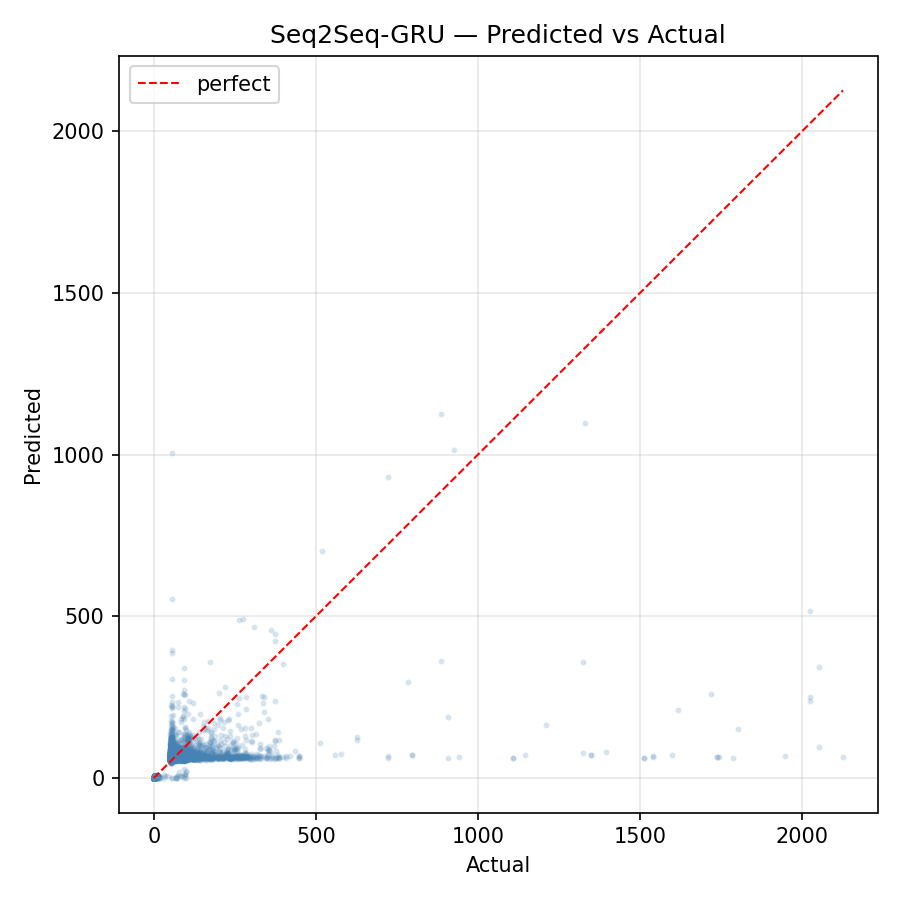
\includegraphics[width=\linewidth]{figures/scatter_s2s_odl.png}
        \caption{Downlink}
    \end{subfigure}
    \hfill
    \begin{subfigure}[t]{0.48\columnwidth}
        \centering
        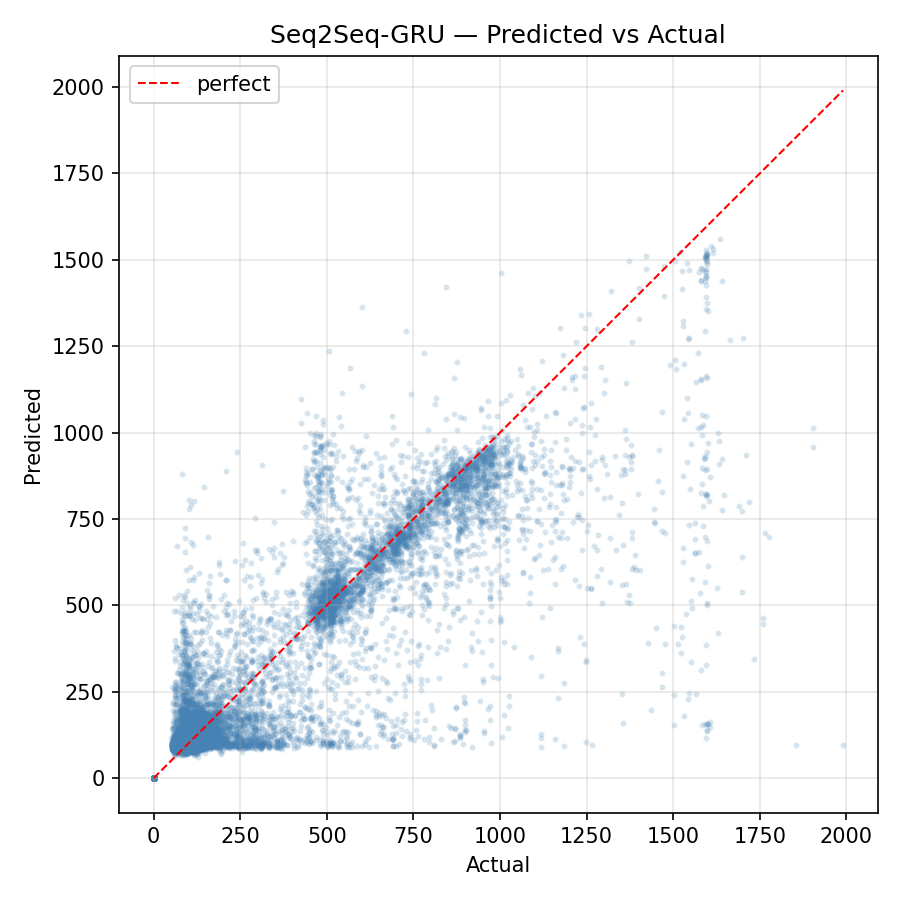
\includegraphics[width=\linewidth]{figures/scatter_s2s_oul.png}
        \caption{Uplink}
    \end{subfigure}

    \caption{Predicted versus actual throughput for the Seq2Seq-GRU model on the OneWeb network. The dashed red line denotes perfect prediction.}
    \label{fig:s2s_oneweb}
\end{figure}

\paragraph{5G.}
5G downlink presents the model's most balanced performance profile. Relative RMSE = 0.796 and relative MAE = 0.870, both below 1.0, confirm the model meaningfully outperforms persistence. RTT R\textsuperscript{2} degrades gradually from 0.318 at $t{+}1$s to 0.196 at $t{+}15$s—a shallow slope that indicates the signal retains some learnable structure even at longer horizons, consistent with a more stable LEO link environment. Jitter shows the clearest horizon-dependence of any target across all datasets: R\textsuperscript{2} falls from 0.820 at $t{+}1$s to 0.166 by $t{+}5$s and plateaus there, indicating a predictability cliff at approximately 5 seconds. Packet loss follows a similar trajectory, dropping from R\textsuperscript{2} = 0.849 at $t{+}1$s to 0.119 at $t{+}15$s. Lag-1 residual autocorrelation is only 0.214, the lowest of the six configurations, suggesting the model captures most of the exploitable serial structure in the 5G downlink signal.

5G uplink is the most challenging configuration overall. Aggregate R\textsuperscript{2} = 0.114, and RTT R\textsuperscript{2} is effectively flat at approximately 0.016--0.018 across all 15 horizons, a sign that the uplink RTT series is close to a random walk at the prediction timescale, with the model offering only marginal improvement over persistence. Jitter degrades from R\textsuperscript{2} = 0.747 at $t{+}1$s to near zero by $t{+}5$s and plateaus, replicating the same predictability cliff seen on the downlink. Packet loss follows an analogous pattern. The low lag-1 autocorrelation of 0.026 indicates that while little serial structure remains unexplained, there was little exploitable structure to begin with, this is a fundamentally noisy signal rather than a mis-specified model.

\begin{figure}[t]
    \centering

    \begin{subfigure}[t]{0.48\columnwidth}
        \centering
        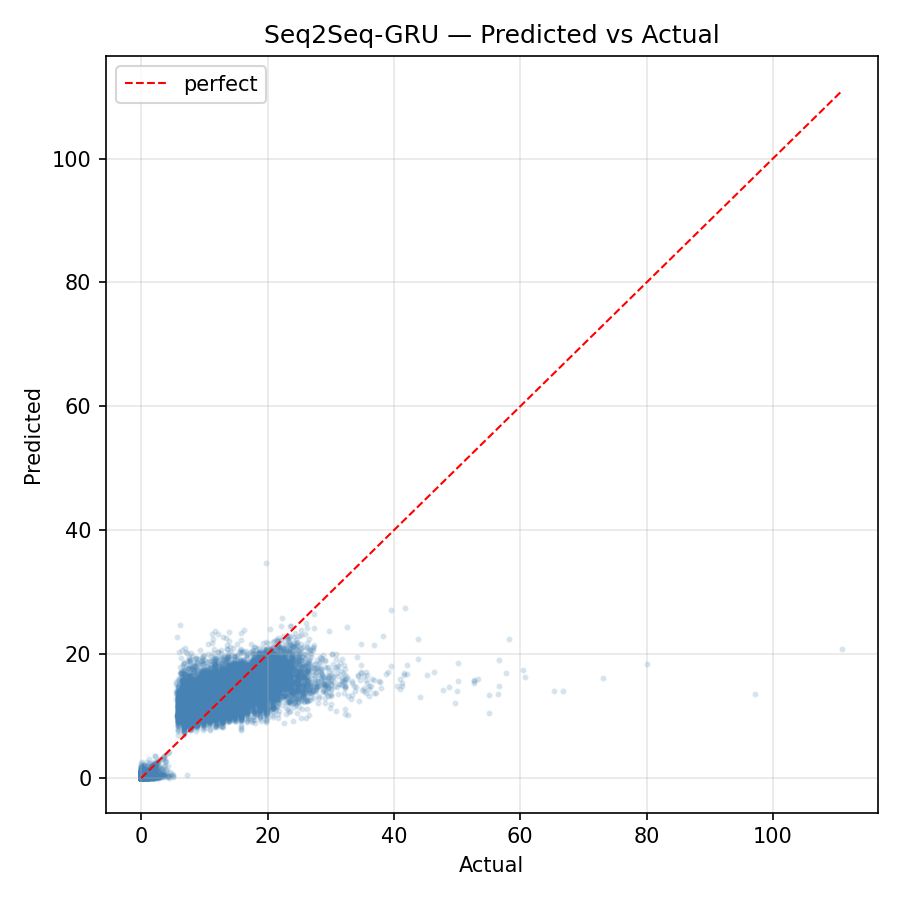
\includegraphics[width=\linewidth]{figures/scatter_s2s_qdl.png}
        \caption{Downlink}
    \end{subfigure}
    \hfill
    \begin{subfigure}[t]{0.48\columnwidth}
        \centering
        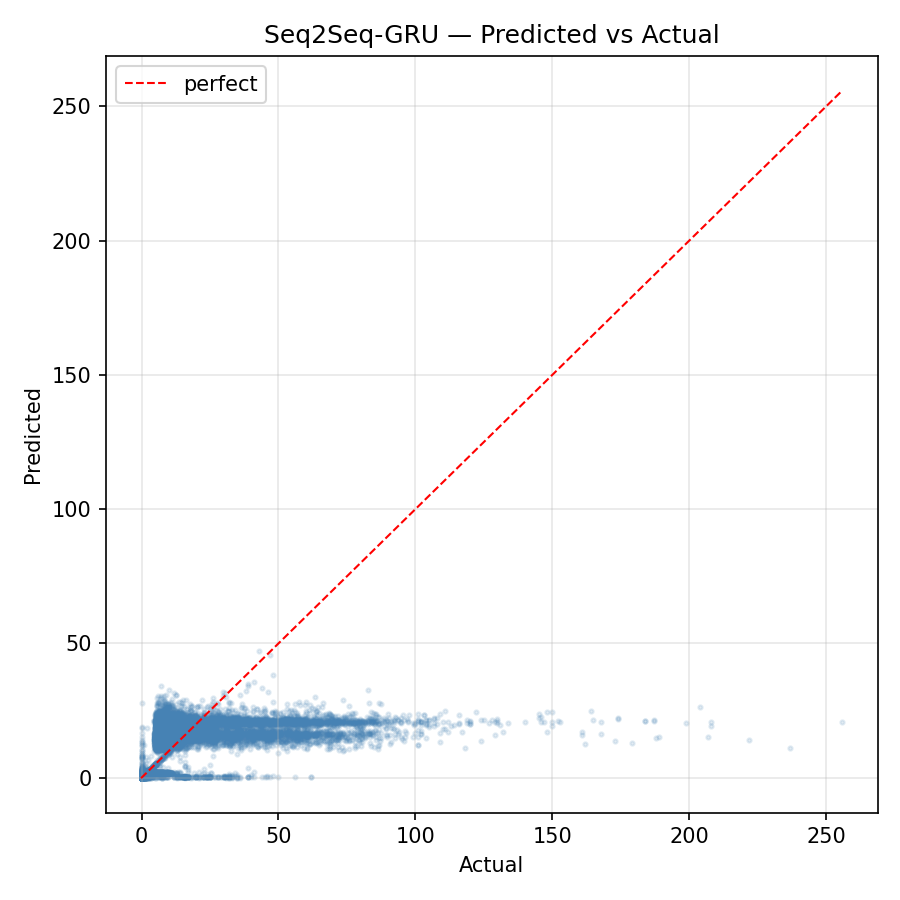
\includegraphics[width=\linewidth]{figures/scatter_s2s_qul.png}
        \caption{Uplink}
    \end{subfigure}

    \caption{Predicted versus actual throughput for the Seq2Seq-GRU model on the 5G network. The dashed red line denotes perfect prediction.}
    \label{fig:s2s_5g}
\end{figure}

\paragraph{Starlink.}
Starlink downlink demonstrates the strongest absolute performance among the three downlink datasets. Relative RMSE = 0.668 and relative MAE = 0.644 indicate the model delivers roughly 33--36\% reduction in error over the persistence baseline, the largest improvement observed across all six configurations. RTT R\textsuperscript{2} begins at 0.728 for $t{+}1$s and decays to 0.555 at $t{+}15$s, a notably shallow degradation compared to OneWeb or 5G, which reflects the richer feature input available for Starlink, including dish-level telemetry and satellite geometry. Jitter and packet loss show the familiar steep initial horizon decay: jitter R\textsuperscript{2} drops from 0.742 to roughly 0.20 by $t{+}5$s; packet loss from 0.791 to 0.306 over the same window. Lag-1 autocorrelation of 0.269 is moderate, indicating some residual temporal structure but substantially less than OneWeb.

Starlink uplink yields aggregate R\textsuperscript{2} = 0.199 and relative RMSE = 0.821, meaning the model improves on persistence by approximately 18\% in RMSE terms. RTT R\textsuperscript{2} declines from 0.381 at $t{+}1$s to 0.318 at $t{+}15$s, a very flat trajectory that suggests low but stable predictability across the horizon. Jitter predictability collapses by $t{+}5$s (R\textsuperscript{2} $\approx -0.06$, slightly below the mean predictor), recovering marginally thereafter. Packet loss degrades from 0.724 to near zero by $t{+}10$s. Lag-1 residual autocorrelation of 0.249 is consistent with Starlink downlink, suggesting the model's residual structure is similar regardless of link direction for this constellation.

\begin{figure}[t]
    \centering

    \begin{subfigure}[t]{0.48\columnwidth}
        \centering
        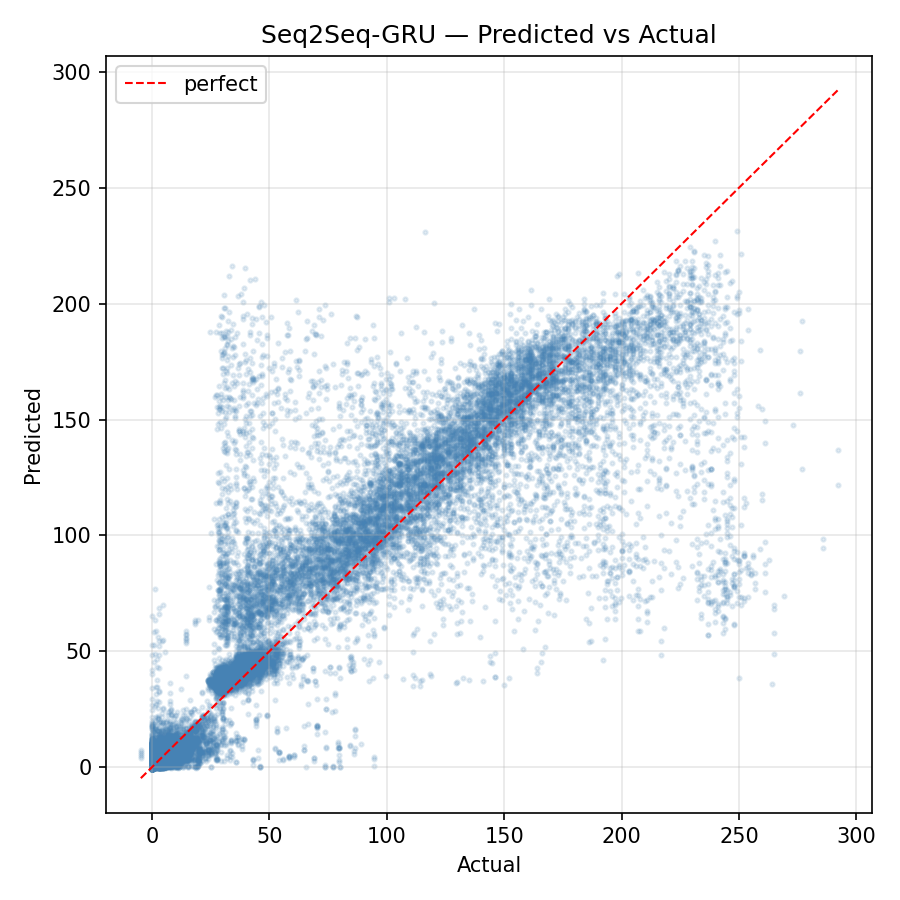
\includegraphics[width=\linewidth]{figures/scatter_s2s_sdl.png}
        \caption{Downlink}
    \end{subfigure}
    \hfill
    \begin{subfigure}[t]{0.48\columnwidth}
        \centering
        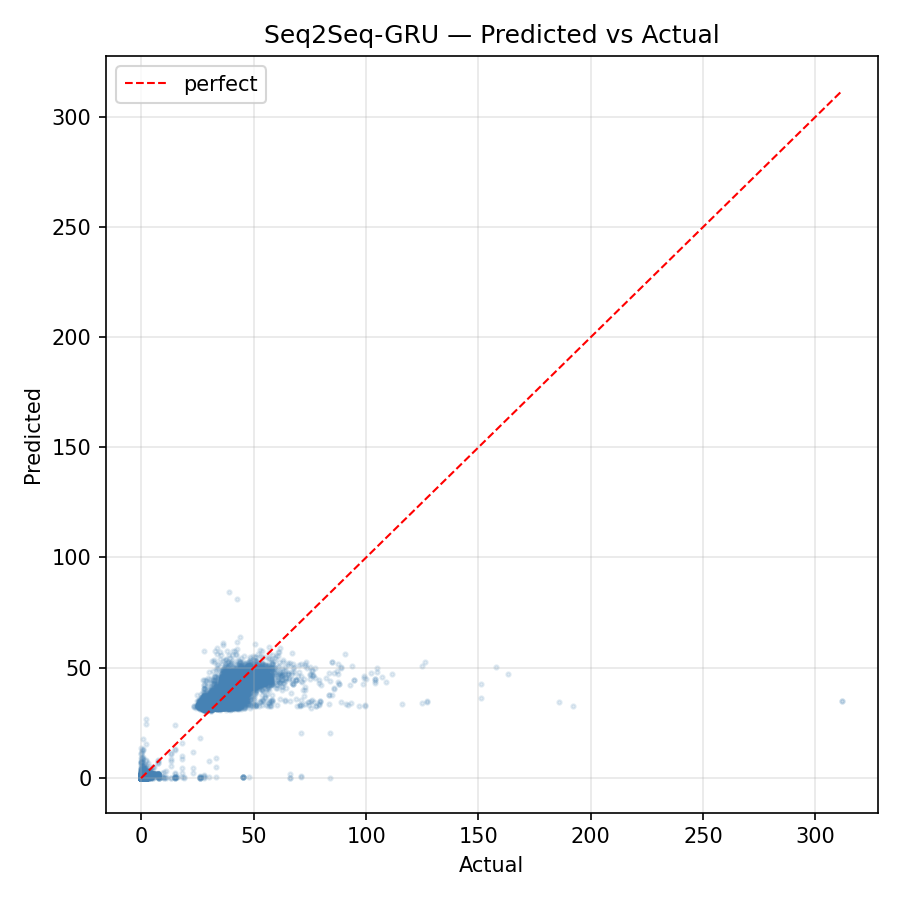
\includegraphics[width=\linewidth]{figures/scatter_s2s_sul.png}
        \caption{Uplink}
    \end{subfigure}

    \caption{Predicted versus actual throughput for the Seq2Seq-GRU model on the Starlink network. The dashed red line denotes perfect prediction.}
    \label{fig:s2s_starlink}
\end{figure}

\paragraph{Cross-Dataset Observations.}
Several patterns emerge consistently across all six configurations and are worth highlighting explicitly.

First, the \emph{1--5 second horizon} is where predictive skill is most concentrated. For jitter and packet loss in particular, R\textsuperscript{2} typically falls by 60--80\% of its initial value within the first five steps, after which it plateaus. This suggests a practical prediction horizon of approximately 3--5 seconds for these targets regardless of constellation. RTT is more forgiving, retaining meaningful R\textsuperscript{2} out to 15 seconds in several configurations.

Second, \emph{richer feature sets improve horizon robustness.} Starlink's feature input, which includes dish-level diagnostics and satellite geometry not available in the OneWeb or 5G experiments, produces shallower R\textsuperscript{2} degradation curves, particularly for RTT. This points to satellite geometry and link-layer state as high-value features for extending the useful prediction horizon.

Third, \emph{high residual autocorrelation (OneWeb DL: 0.760, OneWeb UL: 0.841) signals model headroom}. When lag-1 residual correlation is this large, a more powerful architecture, or additional features capturing handover dynamics, could in principle extract substantially more predictive signal. In contrast, 5G UL's near-zero autocorrelation (0.026) indicates the signal is close to irreducible noise at this timescale, and further architectural complexity is unlikely to help.

Fourth, \emph{interval calibration is uniformly strong} (PICP\textsubscript{95} $= 0.9499$--$0.9500$ across all targets and horizons), confirming that the uncertainty estimates produced by the model are reliable for operational use regardless of point-accuracy limitations.

Fifth, the degenerate jitter and packet loss results on OneWeb uplink (MAE = 0, R\textsuperscript{2} = 1.0) serve as a reminder that aggregate metrics can be misleading when one or more targets exhibit near-constant behavior in the evaluation data.

\subsection{Ablation Study}

The ablation study evaluates the contribution of individual input features to Seq2Seq-GRU performance using a leave-one-out strategy: each feature is dropped in turn and the model is retrained, with the resulting change in MAE, RMSE, and R\textsuperscript{2} relative to the all-features baseline reported as $\Delta$MAE, $\Delta$RMSE, and $\Delta$R\textsuperscript{2}. A positive delta indicates degraded performance when the feature is removed (i.e., the feature was helpful); a negative delta indicates the model actually improves without it. All ablation runs use 30 epochs, consistent input/output lengths of 30 and 15 seconds respectively, and z-score normalization. Results are reported for the downlink direction across all three constellations. Tables~\ref{tab:ablation_oneweb}, \ref{tab:ablation_5g}, and~\ref{tab:ablation_starlink} present the full results sorted by $\Delta$MAE descending. Not present, but a key insight from \cite{liu2025vivisecting} is that time of day plays one of the highest impacts on modeling performance for Starlink. This will carry to any public network that can be effected by user congestion.

\paragraph{OneWeb.}
The OneWeb ablation reveals a clear hierarchy of feature importance, with RTT standing apart as the single most critical input by a substantial margin. Dropping \texttt{rtt\_mean} raises MAE by 0.195 and RMSE by 1.947, roughly four to five times larger than the next most impactful feature, and causes R\textsuperscript{2} to fall by 0.042. This is expected given that RTT is both an input feature and a prediction target: its removal deprives the model of the primary autoregressive signal for its own most predictable output.

More surprising are the features whose removal actually \emph{improves} performance. Dropping \texttt{sinr\_db} reduces MAE by 1.140 and dropping \texttt{elevation\_deg} reduces MAE by 0.945, with both producing marginal or neutral changes in R\textsuperscript{2}. This counterintuitive result suggests that SINR and elevation are adding noise or introducing redundancy with other features rather than providing useful signal at the 30-second input window used in this ablation. It is possible that both features are more informative at coarser temporal resolutions or when modeled jointly with handover events, but at the second-level granularity used here they may introduce distributional variability that the model cannot exploit within 30 training epochs.

Dropping \texttt{packet\_loss\_percent} produces the largest R\textsuperscript{2} degradation ($-0.075$) despite only a modest MAE increase of 0.231, which reflects its disproportionate influence on the packet loss prediction target. Throughput and satellite change contribute moderate positive value ($\Delta$MAE of 0.764 and 0.837 respectively), while time since handover, jitter, and azimuth are roughly neutral to marginally positive.

% ── Ablation Table: OneWeb ───────────────────────────────────────────────────
\begin{table}[ht]
\centering
\caption{Leave-one-out feature ablation for Seq2Seq-GRU on \textbf{OneWeb DL}.
Rows sorted by $\Delta$MAE descending. Positive $\Delta$ = performance degrades without this feature.}
\label{tab:ablation_oneweb}
\setlength{\tabcolsep}{5pt}
\renewcommand{\arraystretch}{1.12}
\small
\begin{tabular}{lrrrrrrr}
\toprule
\textbf{Condition} & \textbf{MAE} & \textbf{RMSE} & \textbf{R\textsuperscript{2}}
  & $\boldsymbol{\Delta}$\textbf{MAE} & $\boldsymbol{\Delta}$\textbf{RMSE} & $\boldsymbol{\Delta}$\textbf{R\textsuperscript{2}} \\
\midrule
All Features (baseline) & 6.845 & 23.555 & 0.221 & --- & --- & --- \\
\midrule
drop \texttt{rtt\_mean}            & 7.040 & 25.502 & 0.179 & $+$0.195 & $+$1.947 & $-$0.042 \\
drop \texttt{satellite\_change}    & 6.008 & 23.999 & 0.200 & $-$0.837 & $+$0.444 & $-$0.021 \\
drop \texttt{packet\_loss\_percent}& 6.076 & 23.951 & 0.146 & $-$0.769 & $+$0.396 & $-$0.075 \\
drop \texttt{throughput\_mbps}     & 6.081 & 24.167 & 0.213 & $-$0.764 & $+$0.612 & $-$0.008 \\
drop \texttt{time\_since\_handover}& 6.178 & 23.635 & 0.214 & $-$0.667 & $+$0.079 & $-$0.007 \\
drop \texttt{jitter\_ms}           & 6.272 & 23.906 & 0.197 & $-$0.573 & $+$0.351 & $-$0.024 \\
drop \texttt{azimuth\_deg}         & 6.289 & 24.108 & 0.214 & $-$0.556 & $+$0.553 & $-$0.006 \\
drop \texttt{elevation\_deg}       & 5.900 & 23.522 & 0.222 & $-$0.945 & $-$0.033 & $+$0.001 \\
drop \texttt{sinr\_db}             & 5.706 & 23.788 & 0.220 & $-$1.140 & $+$0.233 & $-$0.001 \\
\bottomrule
\end{tabular}
\end{table}

\paragraph{5G.}
The 5G ablation presents a notably different picture. The all-features aggregate MAE is 1.103 and most individual drop experiments produce deltas within $\pm$0.013 of that baseline, indicating a relatively flat feature importance landscape where no single feature dominates. The one meaningful exception is \texttt{ping\_rtt\_ms}: dropping it raises MAE by 0.125 and RMSE by 0.095 with an R\textsuperscript{2} decline of 0.034, again reflecting the autoregressive value of including the RTT target as an input feature.

Several features produce slightly negative $\Delta$MAE when dropped, meaning the model performs marginally better without them. These include \texttt{rsrp} ($-0.004$), \texttt{rsrq} ($-0.004$), \texttt{weather\_humidity} ($-0.008$), and \texttt{weather\_pressure} ($-0.001$). The RF signal quality indicators (RSRP, RSRQ) are notable here: despite being standard cellular link-quality metrics, they appear to offer no predictive benefit for 5G QoS over a 15-second horizon, and may even introduce spurious covariance that slightly degrades generalization. Weather features are similarly inert, which is consistent with expectations given that weather dynamics operate on timescales far longer than the 15-second prediction window.

Dropping \texttt{iperf\_jitter\_ms} causes the largest R\textsuperscript{2} drop ($-0.121$) of any 5G feature despite only a small MAE change, confirming that jitter carries disproportionate variance-explaining power for the jitter prediction target even when the aggregate point-error impact is modest. Dropping \texttt{iperf\_throughput\_mbps} marginally \emph{improves} R\textsuperscript{2} by 0.018, suggesting that throughput introduces distributional complexity without improving explained variance, possibly because the 5G uplink signal is near-random at this timescale as established earlier.


% ── Ablation Table: 5G ──────────────────────────────────────────────────
\begin{table}[ht]
\centering
\caption{Leave-one-out feature ablation for Seq2Seq-GRU on \textbf{5G DL}.
Rows sorted by $\Delta$MAE descending.}
\label{tab:ablation_5g}
\setlength{\tabcolsep}{5pt}
\renewcommand{\arraystretch}{1.12}
\small
\begin{tabular}{lrrrrrrr}
\toprule
\textbf{Condition} & \textbf{MAE} & \textbf{RMSE} & \textbf{R\textsuperscript{2}}
  & $\boldsymbol{\Delta}$\textbf{MAE} & $\boldsymbol{\Delta}$\textbf{RMSE} & $\boldsymbol{\Delta}$\textbf{R\textsuperscript{2}} \\
\midrule
All Features (baseline) & 1.103 & 1.655 & 0.263 & --- & --- & --- \\
\midrule
drop \texttt{ping\_rtt\_ms}          & 1.228 & 1.750 & 0.230 & $+$0.125 & $+$0.095 & $-$0.034 \\
drop \texttt{sinr}                   & 1.113 & 1.663 & 0.265 & $+$0.010 & $+$0.008 & $+$0.002 \\
drop \texttt{iperf\_jitter\_ms}      & 1.110 & 1.668 & 0.142 & $+$0.008 & $+$0.013 & $-$0.121 \\
drop \texttt{iperf\_loss\_pct}       & 1.108 & 1.658 & 0.255 & $+$0.006 & $+$0.003 & $-$0.009 \\
drop \texttt{weather\_rain\_rate}    & 1.105 & 1.666 & 0.243 & $+$0.002 & $+$0.011 & $-$0.020 \\
drop \texttt{iperf\_throughput\_mbps}& 1.105 & 1.662 & 0.281 & $+$0.002 & $+$0.007 & $+$0.018 \\
drop \texttt{weather\_pressure}      & 1.103 & 1.656 & 0.268 & $-$0.001 & $+$0.001 & $+$0.005 \\
drop \texttt{rsrp}                   & 1.098 & 1.661 & 0.254 & $-$0.004 & $+$0.007 & $-$0.009 \\
drop \texttt{rsrq}                   & 1.098 & 1.657 & 0.271 & $-$0.004 & $+$0.002 & $+$0.008 \\
drop \texttt{weather\_humidity}      & 1.095 & 1.659 & 0.277 & $-$0.008 & $+$0.004 & $+$0.014 \\
\bottomrule
\end{tabular}
\end{table}

\paragraph{Starlink.}
The Starlink ablation yields the strongest and most interpretable feature importance signal of the three constellations, which is consistent with its larger and richer feature set. Feature impacts span a much wider range than OneWeb or 5G, with $\Delta$MAE values from $-0.285$ to $+5.596$.

\texttt{ping\_server\_rtt\_ms} is by far the most critical feature: its removal raises MAE by 5.596, RMSE by 4.804, and reduces R\textsuperscript{2} by 0.118. This is the largest single-feature impact observed across all three ablation studies and reflects the fact that server-side RTT is both a direct target variable and the highest-autocorrelation input in the Starlink feature set. Removing it forces the model to predict RTT from proxy signals alone.

\texttt{dish\_pop\_ping\_ms} is the second most important feature ($\Delta$MAE = 1.540, $\Delta$R\textsuperscript{2} = $-0.065$), which is meaningful because PoP ping latency is a network-layer metric that captures the ground segment's contribution to end-to-end RTT independently of the space segment. Its high importance confirms that ground infrastructure variability is a material predictor of Starlink QoS, separate from satellite geometry.

\texttt{weather\_rain\_rate} ranks third ($\Delta$MAE = 1.023), which is notably higher than weather impacts observed for 5G. Starlink operates in the Ku/Ka band and is therefore susceptible to rain fade in a way that the LTE-based 5G modem is not, making this finding physically meaningful rather than a statistical artifact.

\texttt{iperf\_jitter\_ms} produces the largest R\textsuperscript{2} degradation in the Starlink ablation ($\Delta$R\textsuperscript{2} = $-0.382$), far exceeding its $\Delta$MAE impact (0.166). As with 5G, this indicates that jitter is a high-variance signal whose removal collapses explained variance on the jitter target while only modestly affecting mean absolute errors on the other targets.

\texttt{satellite\_dtc} Starlink Direct-to-Cell (DTC) is a technology that allows regular smartphones to connect directly to satellites for communication. For modeling, we have 1 if the current satellite supports this and 0 if not. It contributes $\Delta$MAE = 0.222 but a disproportionately large R\textsuperscript{2} drop of $-0.086$, suggesting it carries predictive information for signal variance rather than mean behavior. Conversely, several geometric features, \texttt{elevation\_deg}, \texttt{dish\_obstruction\_fraction}, \texttt{satellite\_handoff}, \texttt{satellite\_age\_s}, and \texttt{dish\_boresight\_azimuth\_deg}, produce neutral or negative $\Delta$MAE, with the boresight azimuth showing the strongest improvement on removal ($\Delta$MAE = $-0.285$). This indicates that not all satellite geometry features contribute at the second-level prediction timescale, and that some may be redundant with \texttt{ping\_server\_rtt\_ms} or \texttt{dish\_pop\_ping\_ms} for the purposes of short-horizon QoS prediction.

% ── Ablation Table: Starlink ─────────────────────────────────────────────────
\begin{table}[ht]
\centering
\caption{Leave-one-out feature ablation for Seq2Seq-GRU on \textbf{Starlink DL}.
Rows sorted by $\Delta$MAE descending.}
\label{tab:ablation_starlink}
\setlength{\tabcolsep}{4pt}
\renewcommand{\arraystretch}{1.12}
\small
\begin{tabular}{lrrrrrrr}
\toprule
\textbf{Condition} & \textbf{MAE} & \textbf{RMSE} & \textbf{R\textsuperscript{2}}
  & $\boldsymbol{\Delta}$\textbf{MAE} & $\boldsymbol{\Delta}$\textbf{RMSE} & $\boldsymbol{\Delta}$\textbf{R\textsuperscript{2}} \\
\midrule
All Features (baseline) & 7.891 & 14.676 & 0.422 & --- & --- & --- \\
\midrule
drop \texttt{ping\_server\_rtt\_ms}         & 13.487 & 19.480 & 0.304 & $+$5.596 & $+$4.804 & $-$0.118 \\
drop \texttt{dish\_pop\_ping\_ms}           & 9.431  & 15.766 & 0.357 & $+$1.540 & $+$1.090 & $-$0.065 \\
drop \texttt{weather\_rain\_rate}           & 8.914  & 15.449 & 0.395 & $+$1.023 & $+$0.773 & $-$0.027 \\
drop \texttt{iperf\_throughput\_mbps}       & 8.270  & 14.776 & 0.375 & $+$0.380 & $+$0.100 & $-$0.047 \\
drop \texttt{weather\_humidity}             & 8.129  & 14.628 & 0.404 & $+$0.239 & $-$0.048 & $-$0.018 \\
drop \texttt{satellite\_dtc}                & 8.113  & 14.599 & 0.336 & $+$0.222 & $-$0.077 & $-$0.086 \\
drop \texttt{azimuth\_deg}                  & 8.093  & 14.790 & 0.421 & $+$0.202 & $+$0.114 & $-$0.001 \\
drop \texttt{distance\_km}                  & 8.078  & 14.725 & 0.405 & $+$0.187 & $+$0.049 & $-$0.017 \\
drop \texttt{iperf\_jitter\_ms}             & 8.057  & 14.744 & 0.039 & $+$0.166 & $+$0.068 & $-$0.382 \\
drop \texttt{weather\_pressure}             & 8.056  & 14.703 & 0.423 & $+$0.165 & $+$0.027 & $+$0.001 \\
drop \texttt{iperf\_loss\_pct}              & 8.044  & 14.854 & 0.345 & $+$0.153 & $+$0.178 & $-$0.077 \\
drop \texttt{dish\_snr}                     & 8.035  & 14.611 & 0.418 & $+$0.144 & $-$0.065 & $-$0.004 \\
drop \texttt{dish\_boresight\_elevation\_deg}& 8.027 & 14.580 & 0.367 & $+$0.136 & $-$0.096 & $-$0.055 \\
drop \texttt{ping\_dns\_rtt\_ms}            & 8.004  & 14.674 & 0.406 & $+$0.114 & $-$0.002 & $-$0.016 \\
drop \texttt{elevation\_deg}                & 7.880  & 14.790 & 0.422 & $-$0.011 & $+$0.114 & $+$0.001 \\
drop \texttt{dish\_obstruction\_fraction}   & 7.865  & 14.665 & 0.420 & $-$0.026 & $-$0.010 & $-$0.002 \\
drop \texttt{satellite\_handoff}            & 7.850  & 14.575 & 0.356 & $-$0.041 & $-$0.101 & $-$0.066 \\
drop \texttt{satellite\_age\_s}             & 7.835  & 14.489 & 0.412 & $-$0.056 & $-$0.187 & $-$0.009 \\
drop \texttt{dish\_boresight\_azimuth\_deg} & 7.606  & 14.655 & 0.428 & $-$0.285 & $-$0.022 & $+$0.007 \\
\bottomrule
\end{tabular}
\end{table}

\paragraph{Cross-Constellation Observations.}
Three findings emerge consistently across all three ablation studies. First, \emph{autoregressive RTT input is the single most important feature in every constellation}, confirming that the prediction problem retains a strong self-predictive component even at 15-second horizons. Second, \emph{jitter's removal consistently produces outsized R\textsuperscript{2} degradation relative to its MAE impact}, indicating it carries disproportionate variance-explaining power for its own prediction target. Third, \emph{several features consistently add no value or mildly hurt performance}, including RF signal quality metrics (SINR for OneWeb, RSRP/RSRQ for 5G) and most coarse satellite geometry features (azimuth, elevation). This suggests that future work could train leaner models with reduced feature sets without sacrificing point accuracy, which would reduce inference overhead and potentially improve generalization to unseen link conditions.

\subsection{Takeaways}

The experiments across three constellations, two link directions, eight model architectures, and a leave-one-out feature ablation converge on a set of findings that characterize the fundamental dynamics of short-horizon QoS prediction over LEO satellite and 5G networks.

\paragraph{Predictability is target-dependent, not network-dependent.} Across all three providers, RTT is the most predictable target and retains meaningful explained variance out to 15 seconds, while jitter and packet loss exhibit a sharp predictability cliff at approximately 3--5 seconds beyond which R\textsuperscript{2} stabilizes near zero. This pattern holds regardless of whether the underlying network is LEO satellite (OneWeb, Starlink) or 5G (5G), suggesting that the temporal structure of QoS metrics is governed more by the physics of the measurement process, RTT integrates over a relatively stable propagation path while jitter and loss reflect bursty, memoryless events, than by the access technology itself. Practitioners designing QoS-aware applications should therefore treat jitter and packet loss predictions beyond a 5-second horizon as unreliable across all three network types evaluated here.

\paragraph{LEO and 5G occupy opposite ends of the predictability spectrum.} Despite sharing the same model architecture and training protocol, performance varies dramatically by provider. OneWeb uplink achieves aggregate R\textsuperscript{2} = 0.918,
while 5G uplink yields R\textsuperscript{2} = 0.114 and OneWeb downlink 0.217. The key differentiator is signal structure: OneWeb uplink RTT exhibits strong autocorrelation that the model exploits effectively, whereas 5G uplink RTT is
effectively a random walk at the prediction timescale (R\textsuperscript{2} flat at $\approx$0.017 across all 15 horizons). Starlink occupies a middle ground, achieving aggregate R\textsuperscript{2} of 0.406 on downlink and 0.199 on uplink. The implication is that prediction feasibility must be assessed per-network and per-direction before deployment; a model that works well on one link configuration may be nearly useless on another even within the same technology class.

\paragraph{Feature richness extends the useful prediction horizon for LEO.} Starlink's 19-feature input, which includes dish-level telemetry, satellite geometry, and ground-segment latency metrics not available for OneWeb or 5G, produces
noticeably shallower R\textsuperscript{2} degradation curves over the 15-second horizon compared to the other two providers. RTT R\textsuperscript{2} declines from 0.728 to 0.555 across the Starlink downlink horizon, a drop of 0.173, versus a decline from 0.706 to $-$0.020 on OneWeb downlink (a drop of 0.726). This strongly implies that satellite geometry and dish-level diagnostics carry predictive information about future link quality that is not available in throughput, SINR, and elevation alone, the feature set shared by OneWeb. Collecting richer telemetry is therefore a practical lever for extending the horizon over which LEO QoS prediction remains actionable.

\paragraph{The most valuable features are network-layer, not physical-layer.} Across all three ablation studies, the features that hurt performance most when removed are network-layer measurements: server-side RTT OneWeb, Starlink, and 5G. Physical-layer indicators, SINR for OneWeb, RSRP and RSRQ for 5G, consistently fail to add predictive value and in several cases mildly degrade performance when included. For Starlink, the ground-segment metric \texttt{dish\_pop\_ping\_ms} ranks second in importance behind server RTT, reinforcing the same conclusion. The practical implication is that QoS prediction models can likely be simplified to a compact set of network-layer inputs without sacrificing accuracy, which reduces deployment overhead and eases integration into existing network monitoring pipelines.

\paragraph{Rain fade is a meaningful predictor for Ku/Ka-band LEO but not for 5G.} The Starlink ablation identifies \texttt{weather\_rain\_rate} as the third most important feature ($\Delta$MAE = 1.023), while weather features are essentially inert for 5G ($|\Delta\text{MAE}| \leq 0.008$ for all weather variables). This is physically consistent: Starlink operates in the Ku and Ka bands, which are susceptible to precipitation-induced attenuation, whereas the sub-6 GHz bands used by 5G's 5G modem experience negligible rain fade. The finding validates the inclusion of real-time weather feeds in Starlink prediction pipelines while simultaneously confirming they are unnecessary overhead for 5G deployments.

\paragraph{Residual autocorrelation identifies where modeling headroom remains.} Lag-1 residual autocorrelation provides a direct diagnostic for unexploited temporal structure. OneWeb downlink (0.760) and uplink (0.841) exhibit the highest values, indicating substantial predictive signal that the current architecture fails to capture, likely due to structured handover dynamics not fully represented in the available features. Starlink (0.269 DL, 0.249 UL) and 5G downlink (0.214) show moderate residual correlation, suggesting partial but incomplete exploitation of available structure. 5G uplink (0.026) is near zero, indicating the signal is close to irreducible noise rather than a modeling shortfall. These diagnostics cleanly separate the networks where improved architectures or richer features would likely yield meaningful gains (OneWeb, Starlink) from those where the prediction problem itself is fundamentally limited by signal unpredictability (5G uplink).

\paragraph{Interval calibration is universally robust, but sharpness is not.} All models across all configurations achieve PICP\textsubscript{95} $\approx$ 0.950, confirming that prediction intervals are reliably calibrated regardless of point-accuracy limitations. However, interval width (MIS) varies considerably: baselines such as GaussianProcess produce intervals three to five times wider than Seq2Seq-GRU on the same dataset, and MIS grows substantially with horizon even as PICP remains fixed. For operational applications that consume uncertainty estimates, such as adaptive bitrate streaming, handover scheduling, or SLA monitoring, well-calibrated but sharp intervals are strictly preferable, and the deep sequence models deliver both.

\paragraph{Degenerate targets require dataset-level scrutiny.} OneWeb uplink jitter and packet loss are effectively constant at zero throughout the evaluation data, yielding trivial R\textsuperscript{2} = 1.0 and MAE = 0. This is a data characteristic, not a modeling achievement, and serves as a reminder that aggregate metrics can be misleading when one or more targets are near-constant in the evaluation split. Any deployment of QoS prediction on LEO networks should include per-target, per-horizon diagnostics and distribution checks on the evaluation data before drawing conclusions from aggregate scores. It also raises a practical question for OneWeb uplink: if jitter and packet loss are negligible in operational conditions, RTT alone may be the relevant prediction target, which simplifies the modeling problem considerably.

\paragraph{Seq2Seq-GRU generalizes well without architectural complexity.} Despite containing fewer than 460{,}000 parameters and training in under 55 epochs, Seq2Seq-GRU matches or outperforms more complex architectures, Transformer, Satellite-ATTENTION, on five of six dataset configurations by MAE and RMSE. The ablation further shows that a reduced feature set (dropping SINR, elevation, and several geometry variables) would not meaningfully harm performance and in some cases would improve it. Taken together, this points to a practical design recommendation for LEO and 5G QoS prediction: a compact recurrent sequence model trained on a curated set of network-layer features is likely to be more reliable and easier to deploy than a larger attention-based model trained on all available telemetry.


\section{Conclusion and Next Steps}\label{sec: conclusion}

From this modeling dynamics study, our next steps are to 1) continue refining the model and 2) integrate the model into multipath QUIC for application evaluation over a SatCom integrated terrestrial network. 

With regards to 1), our modeling work is not done here. As ARA sets up more Starlink user terminals at different locations we can continue to expand our modeling dataset to drive better modeling performance. This includes continuously updating and refining our model, and especially keeping an eye out for new techniques in the research community.

As for 2), this is our next step for this project. Using our top models, we will look to directly see how the model can improve real-time application's quality of experience (QoE). To do this, we will integrate the model into multipath QUIC and conduct experiments using our multipath steering algorithm (which will utilize the model's predicative capabilities) and see how the application's performance increases compared to not using the model. We will also see how the multipath steering algorithm performs as compared to other steering algorithms. 

\bibliographystyle{IEEEtran}
\bibliography{ref}





\end{document}